\documentclass[12pt]{article}
% commonly used packages
\usepackage{calc}
\usepackage{ifthen}
\usepackage{amsmath,amsthm,amsfonts,amssymb}
\usepackage{color,graphicx,overpic}
\usepackage{tabulary}
\usepackage{soul} %for highlight
\usepackage{xcolor} %color definition
\usepackage{sectsty} %change section color
\usepackage{tabulary} % better table
\usepackage[nottoc]{tocbibind}  % for display table and figure
\usepackage{longtable,booktabs,array}
\usepackage{multirow}
\usepackage{float}
% fix Rmd missing package issue
\providecommand{\tightlist}{%
  \setlength{\itemsep}{0pt}\setlength{\parskip}{0pt}}

\newlength{\cslhangindent}
\setlength{\cslhangindent}{1.5em}
\newlength{\csllabelwidth}
\setlength{\csllabelwidth}{3em}
\newlength{\cslentryspacingunit} % times entry-spacing
\setlength{\cslentryspacingunit}{\parskip}
\newenvironment{CSLReferences}[2] % #1 hanging-ident, #2 entry spacing
 {% don't indent paragraphs
  \setlength{\parindent}{0pt}
  % turn on hanging indent if param 1 is 1
  \ifodd #1
  \let\oldpar\par
  \def\par{\hangindent=\cslhangindent\oldpar}
  \fi
  % set entry spacing
  \setlength{\parskip}{#2\cslentryspacingunit}
 }%
 {}
\usepackage{calc}
\newcommand{\CSLBlock}[1]{#1\hfill\break}
\newcommand{\CSLLeftMargin}[1]{\parbox[t]{\csllabelwidth}{#1}}
\newcommand{\CSLRightInline}[1]{\parbox[t]{\linewidth - \csllabelwidth}{#1}\break}
\newcommand{\CSLIndent}[1]{\hspace{\cslhangindent}#1}


\usepackage{graphicx}
\makeatletter
\def\maxwidth{\ifdim\Gin@nat@width>\linewidth\linewidth\else\Gin@nat@width\fi}
\def\maxheight{\ifdim\Gin@nat@height>\textheight\textheight\else\Gin@nat@height\fi}
\makeatother
% Scale images if necessary, so that they will not overflow the page
% margins by default, and it is still possible to overwrite the defaults
% using explicit options in \includegraphics[width, height, ...]{}
\setkeys{Gin}{width=\maxwidth,height=\maxheight,keepaspectratio}
% Set default figure placement to htbp
\makeatletter
\def\fps@figure{htbp}
\makeatother


% use for landscape page
\usepackage{lscape}
\newcommand{\blandscape}{\begin{landscape}}
\newcommand{\elandscape}{\end{landscape}}

% Chinese language support
\usepackage{xeCJK}
% \setCJKmainfont{STKaiti}


% set A4 paper with 2.5cm from left/right and top/bottom
\usepackage[a4paper, margin=2.5cm]{geometry}

% packages for headers
\usepackage{fancyhdr}
\pagestyle{fancy}
\fancyhf{}
\renewcommand{\headrulewidth}{0pt}

% change chapter page number to center bottom
\fancypagestyle{plain}{
  \fancyhf{} 
  \fancyfoot[C]{\thepage}
  \setlength{\headheight}{15pt}
  \renewcommand{\headrulewidth}{0pt}
}

% use double spacing
\usepackage{setspace} \doublespacing

% change abstract title
\usepackage{abstract}

% change section title
\usepackage{sectsty}
\sectionfont{\centering\uppercase}

% change table of content title
\renewcommand*\contentsname{Table of Contents}

% wrap long URL using hyphen
\usepackage{hyperref}
\usepackage{xurl}

% add in figure to list of figures
\usepackage{tocloft}
\newlength{\mylen}

\renewcommand{\cftfigpresnum}{\figurename\enspace}
\renewcommand{\cftfigaftersnum}{:}
\settowidth{\mylen}{\cftfigpresnum\cftfigaftersnum}
\addtolength{\cftfignumwidth}{\mylen}

\renewcommand{\cfttabpresnum}{\tablename\enspace}
\renewcommand{\cfttabaftersnum}{:}
\settowidth{\mylen}{\cfttabpresnum\cfttabaftersnum}
\addtolength{\cfttabnumwidth}{\mylen}

% change caption style
\usepackage{textcase}
\usepackage{caption}
\DeclareCaptionTextFormat{up}{\MakeTextUppercase{#1}}
\captionsetup{justification=centering,textformat=up}
\DeclareCaptionType{equ}[][]


% change citation style
\usepackage[backend=biber,
style=numeric,
citestyle=apa]{biblatex}

%begin document
\begin{document}

% title page
\begin{titlepage}
    \begin{center}
        \vspace*{1cm}

                    \large{\textbf{\uppercase{Generative Adversarial Network (GAN) model in Asset Pricing}}}
        
        \vfill

        by

                    \textbf{\uppercase{Wang Lingjie}}
        
        \vfill

        Honours Thesis in Part Fulfilment for\\
        the Degree of Bachelor of Social Sciences (Honours)

        \vspace{0.8cm}

        %\includegraphics[width=0.4\textwidth]{university}

        Presented to\\
        Department of Economics\\
        National University of Singapore 2021/2022

    \end{center}
\end{titlepage}

\fancyfoot[C]{\thepage}
\setlength{\headheight}{15pt}
\pagenumbering{roman}

% acknowledgement page
\newpage
\renewcommand{\abstractname}{\underline{\uppercase{acknowledgement}}}

            \begin{center}
    \textbf{\underline{\uppercase{ACKNOWLEDGEMENT}}}
\end{center}

I am sincerely thankful for my family and friends who have
accompanied me throughout my undergraduate years. This
thesis would not have happened without your help.

To Dr Denis, I would not have completed this thesis
without your advice and support. Thank you for your
unreserved feedback and comments which materialised this thesis
and pushed me beyond what I thought I could achieve alone.

To my mother who has been taking care me,
thank you for ensuring that I
am well-fed and for putting a roof over my head. Your
unconditional love and support have enabled me to focus on
writing my thesis.
现在是我慈乌反哺以感谢您养育之恩的时候.

To my beloved half - Peiyi, thank you for sharing my worries
and helping to proofread my thesis. Without you, writing
this thesis would be another A-level GP challenge for me.
Thank you for showering me with love and welfare when I was
too busy to take care of myself. I really appreciate
everything you have done for me and I look forward to
disturbing you for a lifetime.

To my friends, thank you for all the fun times we had in
university. Although half of our university years were spent
at home, I still consider us the lucky batch as we managed
to have fun during our freshmen year and created wonderful
memories together in hall. I was also fortunate enough to
experience student exchange in Boston with some of you
before all the lockdowns happened, and it was really an
eye-opening experience to study abroad. 
Not to forget our weekly study group, thank you for all the
bubble tea and snacks, really boosted my grades and weight.
My university life
would not be the same without you all, and I really
appreciate the friendships we forged.

Lastly, to juniors who are considering if you should write a
thesis, I would encourage you to do so. It is definitely not
an easy journey, but I believe the sense of accomplishment
and the research know-how you learned from this process will
be a useful experience for your future endeavors. All the
best!

May God be with us all.

    
\newpage


% abstract page
\renewcommand{\abstractname}{\underline{\uppercase{abstract}}}

% acknowledgement
\newpage
    \begin{centering}

                \begin{abstract}
            An important topic in asset pricing is explaining the variation in expected returns of financial assets. No-arbitrage pricing theory suggests the idea of a pricing kernel that governs asset prices. However, it remains a challenge to estimate the asset-pricing kernel. The difficulties include (1) choosing the right factors, (2) estimating the pricing kernel's functional form, and (3) selecting the right portfolio to estimate the kernel. Recently, Chen et al. (2021) proposed a Generative Adversarial Network (GAN) model that attempts to solve all three challenges in a single setup and claim to achieve the best performance compared to all existing models. This paper seeks to empirically validate Chen et al. (2021)'s research based on the United States stock data with the United Kingdom (UK) London Stock Exchange 1998 - 2017 data. This paper found that the GAN model outperformed the benchmark four-factor model in terms of Sharpe ratio.
        \end{abstract}

        

    \end{centering}

    \vfill

            \textbf{KEYWORDS: Generative Adversarial Network, Asset Pricing, Stochastic Discount Factor, Machine Learning, Deep Learning, Stock Returns}
    
    \vfill

\newpage

% table of contents
    \setcounter{tocdepth}{2}
    \tableofcontents
    \addtocontents{toc}{~\hfill\textbf{Page}\par}

% list of tables and figures
\listoffigures
\addtocontents{lof}{~\hfill\textbf{Page}\par}
\listoftables
\addtocontents{lot}{~\hfill\textbf{Page}\par}
\newpage

% change page number to top right
\fancyhf{}
\fancyhead[R]{\thepage}
\setlength{\headheight}{15pt}
\pagenumbering{arabic}

% put in the rest of body here
\hypertarget{introduction}{%
\section{Introduction}\label{introduction}}

\thispagestyle{plain}

An important goal in asset pricing is to explain the variation
in expected returns of financial assets.
No-arbitrage pricing theory suggests the idea of a pricing
kernel, also known as the stochastic discount factor (SDF),
that governs asset prices.
The literature on determining the appropriate form of the
SDF has a long history and perhaps one of the most extensive
analyses in finance.
However, it remains a challenge to estimate the pricing
kernel. There are three challenges in estimating the
asset-pricing kernel:
(1) choosing the right factors (data features) to
estimate the pricing kernel,
(2) estimating the functional form of the pricing
kernel and,
(3) selecting the right portfolio (combination of
individual assets) to estimate the pricing kernel.

Factor models such as Fama \& French (1993)'s three-factor model
and Carhart (1997)'s four-factor model
constructed different factors based on empirical
findings and estimated the pricing kernel through a linear
combination of these constructed factors.
These factor models have been performing well empirically,
and are considered the benchmark for assets pricing models.
Besides exploring various new possible factors,
recent literature also attempts to estimate the pricing
kernel using non-linear and non-parametric methods.
For example, Gu et al. (2020) found that neural network models
outperform linear models in estimating the pricing kernel.
Furthermore, Gu et al. (2021) also realised that imposing
economic theory onto machine learning models can
improve model performance further.

With reference to existing literature, Chen et al. (2021) proposed a
Generative Adversarial Network (GAN) model that imposes the
no-arbitrage condition in the neural network model.
GAN models are a class of neural network frameworks which
consist of two competing network models in a zero-sum game.
A discriminative neural network attempts to price the asset
prices using no-arbitrage condition, while a generative neural network attempts
to increase the pricing error through different combinations of
assets and factors.
Through the alternating training, the discriminative
neural network estimates the functional form of
the pricing kernel while the
generative network constructs portfolios
that no-arbitrage condition is least able to explain, thus solving the three
problems in empirical asset pricing theory in a single setup.
As compared to previous research that focused on firm
characteristics data, Chen et al. (2021) included
macroeconomic data using long short-term memory (LSTM), a
class of neural network architecture commonly used in
predictions with a time series structure. Their findings
have shown that the inclusion of macroeconomic data did
enhance the model performance.
Therefore, Chen et al. (2021) analyses have outperformed all
previous models in Sharpe ratio, explained variation and
pricing errors.

However, similar to most literature, Chen et al. (2021)'s
research focus solely on the United States (U.S.) market.
In fact, Karolyi (2012) pointed out that only few papers in top
finance journals have explored the model performance in
non-U.S. markets.
The lack of comparison of model performance on non-U.S.
markets thus motivates this paper to empirically validate the
external validity of Chen et al. (2021)'s research with the
United Kingdom London Stock Exchange data from 2011 to 2021.
This paper is organised as follows: Section 2 provides the
literature review, Section 3 explains the methodology,
Section 4 and 5 goes in-depth on the model training and
evaluation metrics, Section 6 and 7 explains the data and
empirical findings.
This paper will end with discussion in Section 8 and
finally, conclusion in Section 9.
Overall, this paper concludes that the GAN model outperformed
benchmark four-factor model when evaluated against the Sharpe
ratio.
Replication files are available on the author's GitHub
account
\href{https://github.com/lingjie00/asset_pricing}{github.com/lingjie00/asset\_pricing}.

\hypertarget{literature-review}{%
\section{Literature Review}\label{literature-review}}

\thispagestyle{plain}

The literature on determining the appropriate form of the
SDF has a long history and perhaps is one of the largest
analysis in finance. The first asset-pricing model proposed by
Sharpe (1964), Lintner (1965) and
Mossin (1966) in the 1960s was the
Capital Asset Pricing Model (CAPM).
CAPM explains the variation in asset
returns with the assets' exposure to market risk.
The exposure is measured by a linear pricing kernel against
a wealth portfolio which includes all possible asset
classes. However, in reality, broad stock market index is
commonly used as a proxy for the wealth portfolio.
The resultant regression coefficient in this single-factor
model is coined as ``beta'', and investors continued to use
``beta'' as a measure of the systematic risk of assets.

Ross (1976) proposed the arbitrage pricing theory
(APT) and shown that if returns are generated by a linear
factor model, there is a SDF linear in factors that prices
the returns. However, the exact factors remained unknown.
Fama \& French (1993) proposed their version of candidate
factors based on the APT and derived a three-factor model that
expands on the CAPM model by including size and value
factors.
Fama \& French (1993) found that small market capitalisation
stocks and low-value stocks outperformed the market, and
including the size and value factors improves the
performance of the CAPM model.
The size factor is the difference in returns between the
smallest and largest stocks measured by market capitalisation.
On the other hand, the value factor is the difference in
returns between the cheapest and
most expensive stocks measured by price to book ratio.
Carhart (1997) built on the three-factor model
to include a momentum factor: the difference
in returns between the best and worst-performing stocks.
Fama \& French (2015) later expanded on the three-factor model to
include profitability and investment. The profitability
factor is the difference in returns between stocks with high
and low operating profitability, and the investment factor is
the difference in returns between high and low capital
investment stocks. The three, four, and five factor models
have been a benchmark for asset pricing models and
remain relevant today.
In recent years, different research papers have attempted to
find new factors to improve the factor model performance.
The term ``factor zoo'' was used by Feng et al. (2020) to
describe the hundreds of factors proposed over the years in
the literature.
Feng et al. (2020) and Freyberger et al. (2017)
investigated a wide range of such proposed factors and found
that only a handful are
statistically significant in explaining the asset returns.

The factor models mentioned earlier have explored different
factors while assuming a linear functional form for the SDF.
Recent literature attempt to estimate the SDF
with non-linear, non-parametric models such as decision tree-based methods and
neural network models. Non-parametric models do not require
a priori knowledge of the SDF's functional form and
allow estimation of flexible non-linear functions.
Moreover, Freyberger et al. (2017) show that
non-linear relationships are essential in SDF estimation.
Gu et al. (2020) compared different
machine learning models and show that tree and neural
network models marginally outperform linear models,
with the neural network model emerging as the best performing model,
measured by the out-of-sample \(R^2\).

Traditional machine learning models do not
consider economic theories during estimation.
Gu et al. (2021) found that imposing
constraints based on economic theory can further improve
the neural network models.
Furthermore, Chen et al. (2021) imposed a no-arbitrage condition on neural
networks through a generative adversarial network (GAN)
model.

Goodfellow et al. (2014) first introduced GAN models for image recognition tasks,
and GAN models continue to be heavily used in image and video tasks,
as suggested by S \& Durgadevi (2021)'s recent survey.
GAN models differ from classical neural network models by including two
competing neural networks in a zero-sum game. In the context
of Chen et al. (2021) and this paper, one of the neural
networks will price assets through no-arbitrage condition while the
other neural network will attempt to find factors and
mispriced assets to increase pricing error.
This paper will explain the GAN model in detail in the methodology section.

Consumption-based asset pricing is an alternative approach
that derives SDF directly from a utility function. However,
Campbell \& Cochrane (2000) show that the consumption-based model
cannot account for the time-varying
nature of SDF, resulting in poor performance compared to
the factor models. Therefore, this paper focuses on
factor models.

Current literature estimates SDF solely based on the
firm characteristics data. However,
Pelger \& Xiong (2020) found that
including macroeconomic data can further improve the
performance of machine learning models, which is also
evident in Chen et al. (2021)'s results.
Chen et al. (2021) included a recurrent neural network with
long short-term memory (LSTM) architecture in the GAN model
to capture the time series dynamics of the macroeconomic data.
Hochreiter \& Schmidhuber (1997) first proposed the LSTM architecture, and a recent
review on the applications of LSTM by Houdt et al. (2020)
found that LSTM is still commonly used in sequence data to
capture dynamics in data, such as language-related tasks.
This paper will also explain the different LSTM components
in the methodology section.

The main contribution of this paper is in examining the
external validity of Chen et al. (2021)'s model using the
United Kingdom (U.K.) London Stock Exchange (LSE) data.
Karolyi (2012) found that most
empirical papers consider the data-rich United States, with
only around 20\% of the papers in top finance journals
investigating countries outside the United States (U.S.).
Likewise, Chen et al. (2021) model was also
trained based on the U.S. data.
Therefore, this paper explores the model performance in a
different context, such as the U.K. market.
There are several works of literature done on LSE data,
but none answers the question this paper seeks to address.
Bhatnagar \& Ramlogan (2012) and
Korajczyk \& Viallet (1989) focus only on
linear factor models, while Tobek \& Hronec (2018)
forecast asset prices without considering economic theories.
Therefore, one of the critical contributions of this paper
is to provide insights into the potential benefits advanced
models can bring to the empirical asset pricing of UK
securities.

\hypertarget{methodology}{%
\section{Methodology}\label{methodology}}

\thispagestyle{plain}

This chapter focuses on explaining the empirical approach used in this
paper. First, we present the no-arbitrage asset-pricing
model that is the foundation of our base model: the
Fama-French factor model and the GAN model. Next, we
expand the no-arbitrage condition to construct a pricing
loss function used in the GAN model. Then, we describe a
simple feed-forward neural network before exploring a
recurrent neural network model that considers data dynamics.
Following that, we explain the GAN model, which
consists of two neural network models competing based on the
pricing loss function and end the chapter
with an explanation for the Fama-French factor model.

Training neural network models is an empirical challenge.
Regularization techniques are commonly used in machine
learning to prevent over-fitting and improve model training
results. Chen et al. (2021) adopted a dropout strategy proposed
by Srivastava et al. (2014).
This paper further includes early stopping rules introduced
by Yao et al. (2007).
The discussion on neural networks presented in this section
is referenced from the
Hands-On Machine Learning with Scikit-Learn and TensorFlow
by Géron (2017).

\hypertarget{no_arbitrage}{%
\subsection{No-arbitrage asset-pricing model}\label{no_arbitrage}}

The no-arbitrage asset pricing model assumes the existence
of an asset independent, time-dependent pricing kernel, also known as a stochastic
discount factor (SDF) \(M_t\), such that there is no excess
return in expectation.
Let \(R_{t+1, i}\) denote the asset \(i\)'s return in
time \(t+1\) and \(R^f_{t+1}\) as the return of a risk-free asset.
The excess return is then defined as \(R^e_{t+1, i} := R_{t+1, i} - R^f_{t+1}\). Summarising the no-arbitrage
condition, we have the equation
\[
E_t[M_{t+1} R^e_{t+1, i}] = 0.
\]

SDF can be expressed as an affine transformation of a
mean-variance efficient tangency portfolio.
The mean-variance efficient frontier refers to the maximum
possible balance between the mean excess returns and risk
factor, measured by the variance of the
excess returns. A portfolio that maximises mean-variance
efficiency is considered as a tangency portfolio.
Let \(\mathbf{\omega}_t\) denote the SDF weights used to
construct the tangency portfolio based on all the assets in
the market, and
\(F_{t+1} := \mathbf{\omega}_t^T R^e_{t+1}\) denote the tangency
portfolio.
Using the covariance formula
\(E(XY)=E(X)E(Y) + Cov(X, Y)\) and correlation formula
\(E(XY) = E(X)E(Y)+\rho(X, Y)\sigma(X)\sigma(Y)\),
we have \(E(M_{t+1})E(R^e_{t+1, i}) = -\rho(M_{t+1}, R^e_{t+1, i})\sigma(M_{t+1})\sigma(R^e_{t+1})\). Since
\(\rho(\cdot)\in(0, 1)\), we can express the bounds of the
excess return as a function of the risk of the asset,
forming the mean-variance frontier, illustrated in
figure \ref{fig:mvf}

\[
|E_t(R^e_{t+1, i})| \leq \left(\frac{\sigma_t(M_{t+1})}
{E_t(M_{t+1})}\right)\sigma_t(R^e_{t+1}).
\]

\begin{figure}
\centering
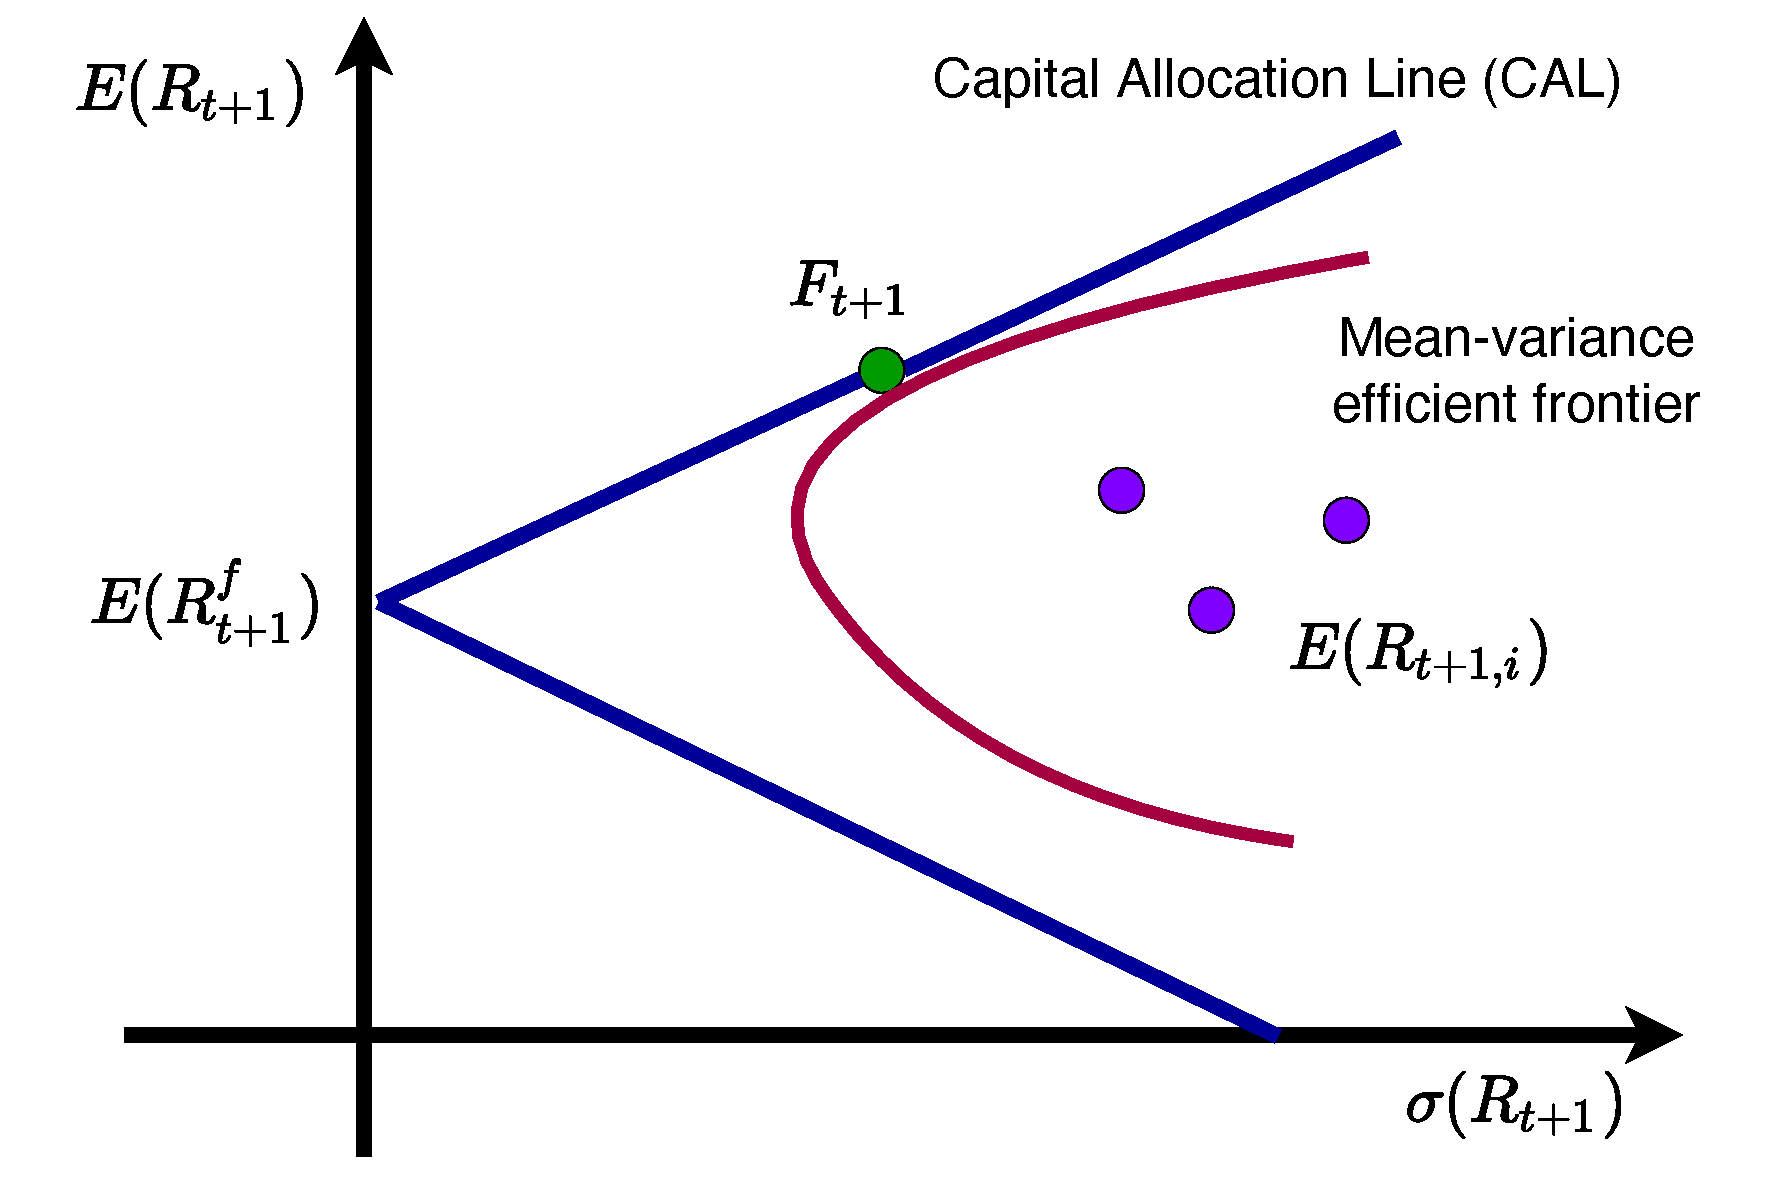
\includegraphics[width=0.5\textwidth,height=\textheight]{./src/mvf}
\caption{\label{fig:mvf} Mean-variance frontier}
\end{figure}

Since the tangency portfolio occurs at the mean-variance
frontier where \(\rho(M_{t+1}, F_{t+1})=-1\),
it is perfectly correlated to the SDF
which is given by an affine transformation of the SDF
(\(M_{t+1} = a - b F_{t+1}\)). Since any
mean-variance efficient return carries all the pricing
information, without loss of generality,
we consider one of the possible \((a, b) = (1, 1)\)

\[
M_{t+1} = 1 - F_{t+1} = 1 - \mathbf{\omega}_t^T R^e_{t+1}.
\]

Therefore, the no-arbitrage condition reduces the
asset-pricing problem into estimating an SDF weight function
\(\omega\) such that the following equation holds. We will
use this relationship to construct our loss function that
trains the GAN model

\[
E\left[\left(1-\mathbf{\omega}_t^T R^e_{t+1}\right)R^e_{t+1, i}\right] = 0.
\]

\hypertarget{loss_function}{%
\subsection{Pricing loss function}\label{loss_function}}

The no-arbitrage condition reduces the asset pricing problem
into estimating the SDF weight function \(\omega\).
This paper assumes \(\omega\) is a function of
macroeconomic data \(I_t\) and firm characteristic
data \(I_{t, i}\).
However, suppose the no-arbitrage condition
alone is insufficient to explain the differences in asset
prices. In that case, we can define a function \(g(I_t, I_{t, i})\)
that selects firm characteristic and assets and output some factor
unexplained by the no-arbitrage
to price the assets. The relationship between \(\omega(I_t, I_{t, i})\) and \(g(I_t, I_{t, i})\) can be described by the
following equation. We define this as our pricing loss
function. The pricing loss function can be viewed as a
competition between the no-arbitrage condition and an
alternative theory that explains the variation in
asset excess returns, which is the key in building the
GAN model proposed by Chen et al. (2021)

\[
E\left[\left(1-\omega(I_t, I_{t, i})^T R^e_{t+1}\right)R^e_{t+1, i}
g(I_t, I_{t, i})
\right] = 0.
\]

\hypertarget{nn_model}{%
\subsection{Neural network model}\label{nn_model}}

A neural network model is a flexible non-parametric
model that is able to recover effectively the non-linear
relationships, including the interaction effects, between
input and output data.
In this paper, we build two neural network models to (1) model
the stochastic discount factor (SDF) weight and (2) model
factors unexplained by the no-arbitrage condition. The \protect\hyperlink{gan_model}{GAN
model} section provides an in-depth explanation of
these two neural networks.
Each of the two neural network models combines feed-forward
and recurrent neural networks. We first explain the
standard feed-forward
neural network before expanding to the recurrent neural network
in long short-term memory (LSTM)
architecture under \protect\hyperlink{LSTM_model}{subsection 3.4}. Regularization techniques are
employed to minimise model over-fitting and are explained
under \protect\hyperlink{model_training}{subsection 4.1}.

\hypertarget{feed-forward-neural-network}{%
\subsubsection{Feed-forward neural network}\label{feed-forward-neural-network}}

A standard feed-forward neural network (FFN) consists of one input
layer, one or multiple hidden layer(s) and one output layer.
In essence, FFN performs a linear combination of covariates
before passing the intermediate output to a non-linear function.
The output from the non-linear function is then linearly
combined again, and the procedure repeats until the output
layer. This paper first illustrates this relationship using
Figure \ref{fig:feedforward} before introducing the
individual components.

The first layer in Figure \ref{fig:feedforward} is
the \emph{input layer}. The number of input units in the input
layer corresponds to the number of covariates available.
Therefore, an input data \(\mathbf{X} = (X_1, X_2, \cdots, X_p)\)
with \(p\) covariates will have \(p\) input units in the input
layer. The input data in this paper includes
both macroeconomic factors and firm characteristics data.

The second layer in Figure \ref{fig:feedforward} is the
\emph{hidden layer}. The input units are linked to the hidden
layer as a directed acyclic graph (DAG). Each hidden unit
will first linearly combine the input units before
passing the intermediate output to a non-linear function
\(h(\alpha_{0m} + \mathbf{\alpha}^T_m\mathbf{X})\),
where \(h(\cdot)\) is the non-linear function, \(m = 1, \cdots, M\) is the \(m\)th hidden unit, and \(\alpha\) is the
weights in the hidden unit.
The output in the hidden units is a non-linear
transformation of the input units.
Although the figure only shows a single hidden layer,
there might be multiple hidden layers in practice, forming a
deep neural network. The output of the hidden units will be
passed as the input to the next hidden layer, and the
procedure repeats.

The third and final layer in Figure \ref{fig:feedforward}
is the \emph{output layer}. The number of output units in the
output layer depends on the nature of the predicted
variable. For example, in the case of a continuous \(Y\), we
have one output unit and in the case of categorical \(Y\) the
number of output units will follow the number of categories.
In the continuous \(Y\) case, the
outputs from the hidden units are linearly combined to
produce a single value as the final output of the FFN.

\begin{figure}
\centering
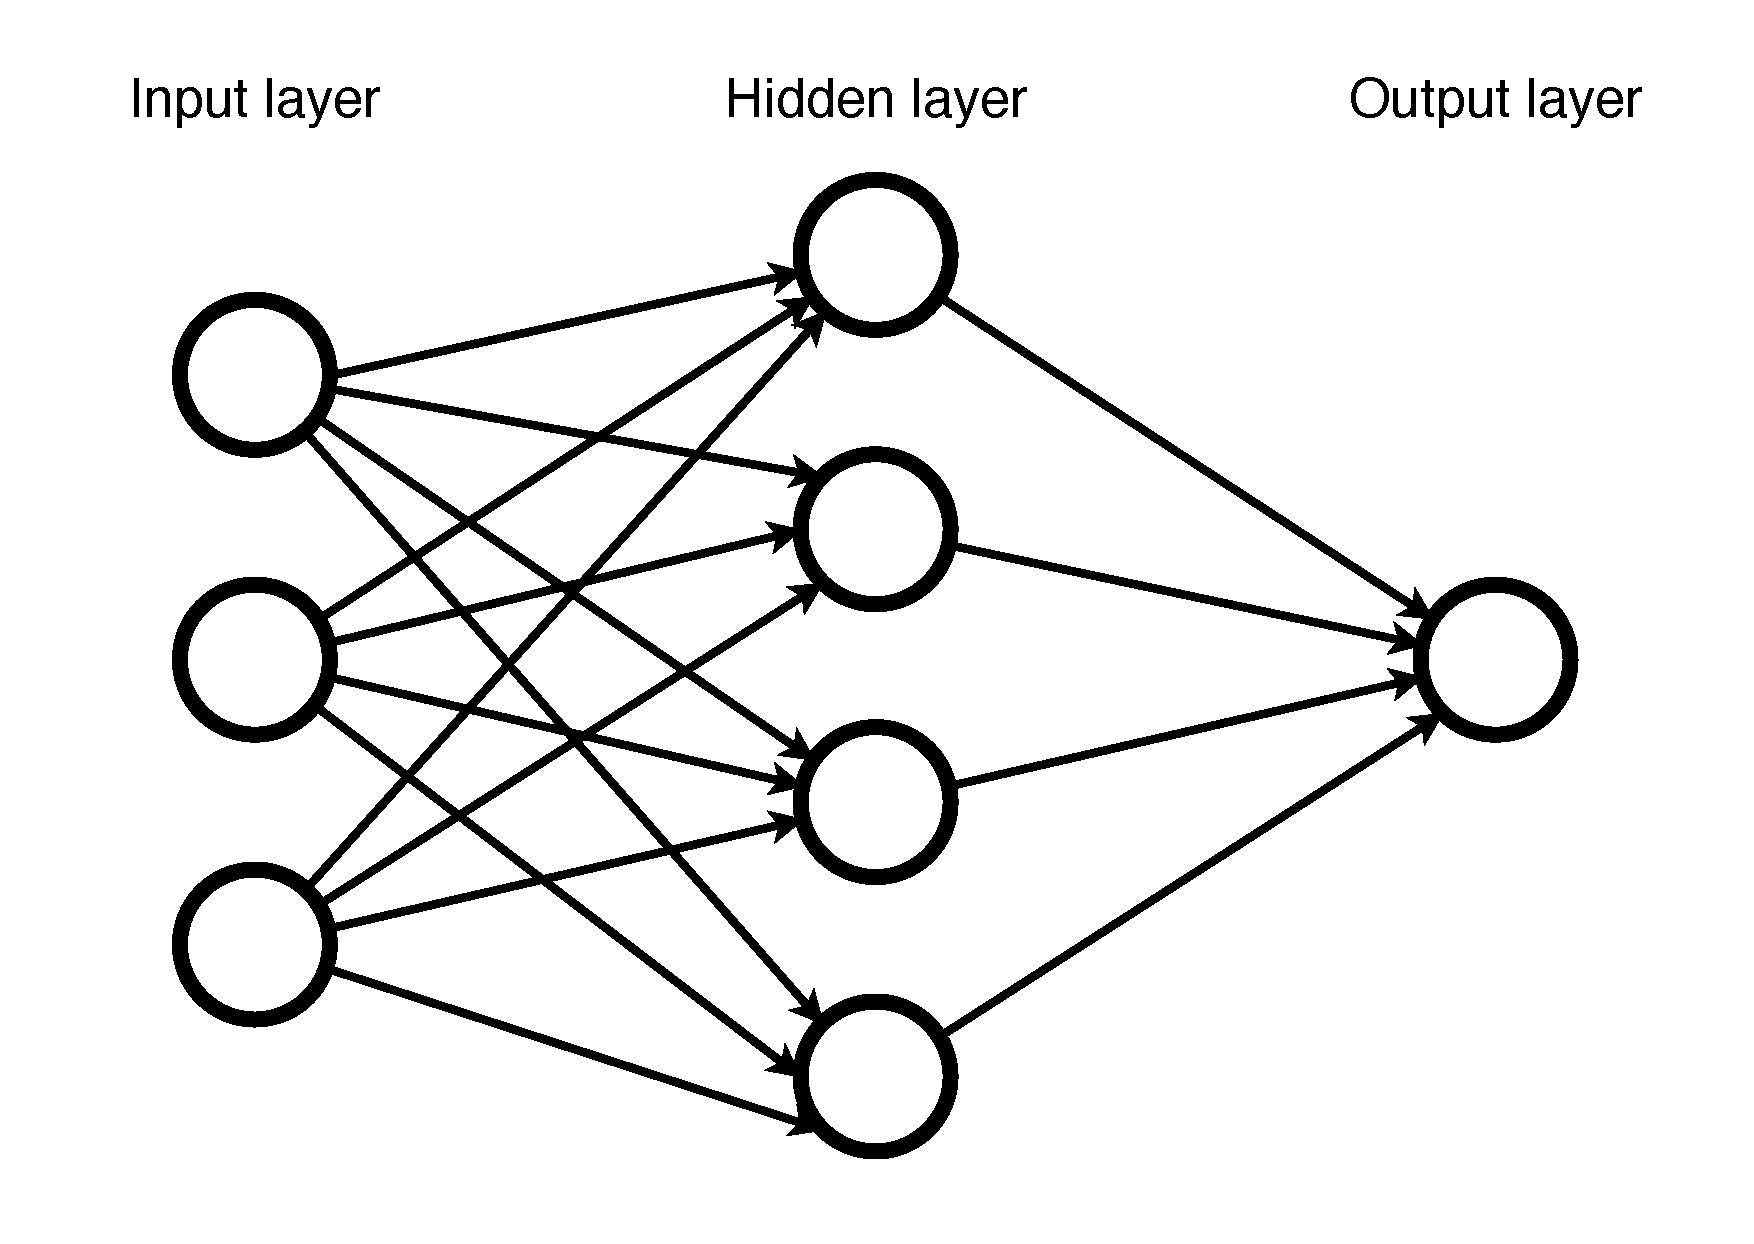
\includegraphics[width=0.7\textwidth,height=\textheight]{./src/feedforward}
\caption{\label{fig:feedforward} Feed-forward neural network}
\end{figure}

\hypertarget{network-components}{%
\subsubsection{Network components}\label{network-components}}

Let \(\mathbf{X}\) be the vector of inputs, \(y\) be the numeric
output being predicted when \(Y\) is continuous, \(M\) be the
total number of hidden units, \(\alpha\) be the constants in the
hidden units and \(\beta\) be the weights in the output unit.
The neural network structure can be summarized with the
following equations

\begin{align*}
    Z_m &= h(\alpha_{0m} + \mathbf{\alpha}^T_m\mathbf{X}), ~m
    = 1, \cdots, M,\\
    \mathbf{Z} &= (Z_1, Z_2, \cdots, Z_m),\\
    y &= \beta_{0} + \mathbf{\beta}^T \mathbf{Z}.
\end{align*}

\hypertarget{activation-function}{%
\subsubsection{Activation function}\label{activation-function}}

Multiple activation functions are used in the literature.
This paper uses one of the most commonly
used activation functions known as rectified linear unit
(ReLU), shown in Figure \ref{fig:relu}. \(ReLU(x) := \max(x, 0)\) effectively removes the negative values.
Nair \& Hinton (2010) shown in their paper that ReLU
improves the convergence rate of stochastic gradient descent
compared to other activation functions such as the logistic
function.

\begin{figure}

{\centering \includegraphics[width=0.7\linewidth]{thesis_files/figure-latex/relu-1} 

}

\caption{Rectified linear unit (ReLU) activation function}\label{fig:relu}
\end{figure}

\hypertarget{loss-function}{%
\subsubsection{Loss function}\label{loss-function}}

After the data is passed from the input layer to the output
layer, network predictions are evaluated using an
appropriate loss function.
One commonly used loss function is
the squared loss \(L(y, \hat{y}) = (y-\hat{y})^2\).
This paper implements a custom pricing loss
function described in the pricing loss
function under \protect\hyperlink{loss_function}{subsection 3.2}.

\hypertarget{back-propagation}{%
\subsubsection{Back-propagation}\label{back-propagation}}

After the loss is calculated, a back-propagation training
algorithm is then used to train the network.
Back-propagation algorithm minimises a given loss function
by updating the weights and constant terms in the network model
through gradient descent methods. This paper adopted
adaptive moment estimation (Adam) as the optimizer as
described in \protect\hyperlink{adam}{subsection 4.1}.

\hypertarget{LSTM_model}{%
\subsection{Long short-term memory network architecture}\label{LSTM_model}}

A recurrent neural network (RNN) is a class of neural
networks that considers the past data in future prediction
and hence is particularly suited for the prediction of time
series data.
Long Short-Term Memory (LSTM) is a sub-class of RNN that
considers more extended dynamics through a gate controlling
system.
We focus our discussion here on LSTM.
In contrast to a feed-forward network that receives only
input data \(\mathbf{x}_{(t)}\) at time \(t\),
an LSTM also gets a short term state
\(\mathbf{h}_{(t)}\) and a long term state \(\mathbf{c}_{(t)}\).

As shown in figure \ref{fig:lstmcell}, the long term state
\(\mathbf{c}_{(t-1)}\) from the previous iteration travels
through a forget gate and an input
gate before being passed through to the next iteration.
The long term state \(\mathbf{c}_{(t)}\) is also being passed
as a short term state \(\mathbf{h}_{(t)}\) through an output
gate (which is also the output of the cell \(\mathbf{y}_{(t)}\)).
The gates are being controlled by the functions
\(\mathbf{f}_{(t)}, \mathbf{i}_{(t)}, \mathbf{o}_{(t)}\), with
logistic activation functions that produce \(1\) to keep the
gate open and \(0\) to close the gate. The decision on the
gates is based on the input data \(\mathbf{x}_{(t)}\) and
the short term state \(\mathbf{h}_{(t)}\). The function
\(\mathbf{q}_{(t)}\) takes in the data and short term state to
be combined with the long term state.
Summarising the LSTM computation, we have the following
equations. \(\mathbf{W}_{x\cdot}\) are the weights for
\(\mathbf{x}_{(t)}\), and \(\mathbf{W}_{h\cdot}\) are the weights
for \(\mathbf{h}_{(t-1)}\) and \(\mathbf{b}_i\) are the constants for
\(i\) layers, \(\otimes\) are element-wise multiplication.
Therefore, using an LSTM neural network layer allows the GAN
model to extract long term dynamics from macroeconomics data
without specifying the number of lags as a hyper-parameter.

\begin{figure}
\centering
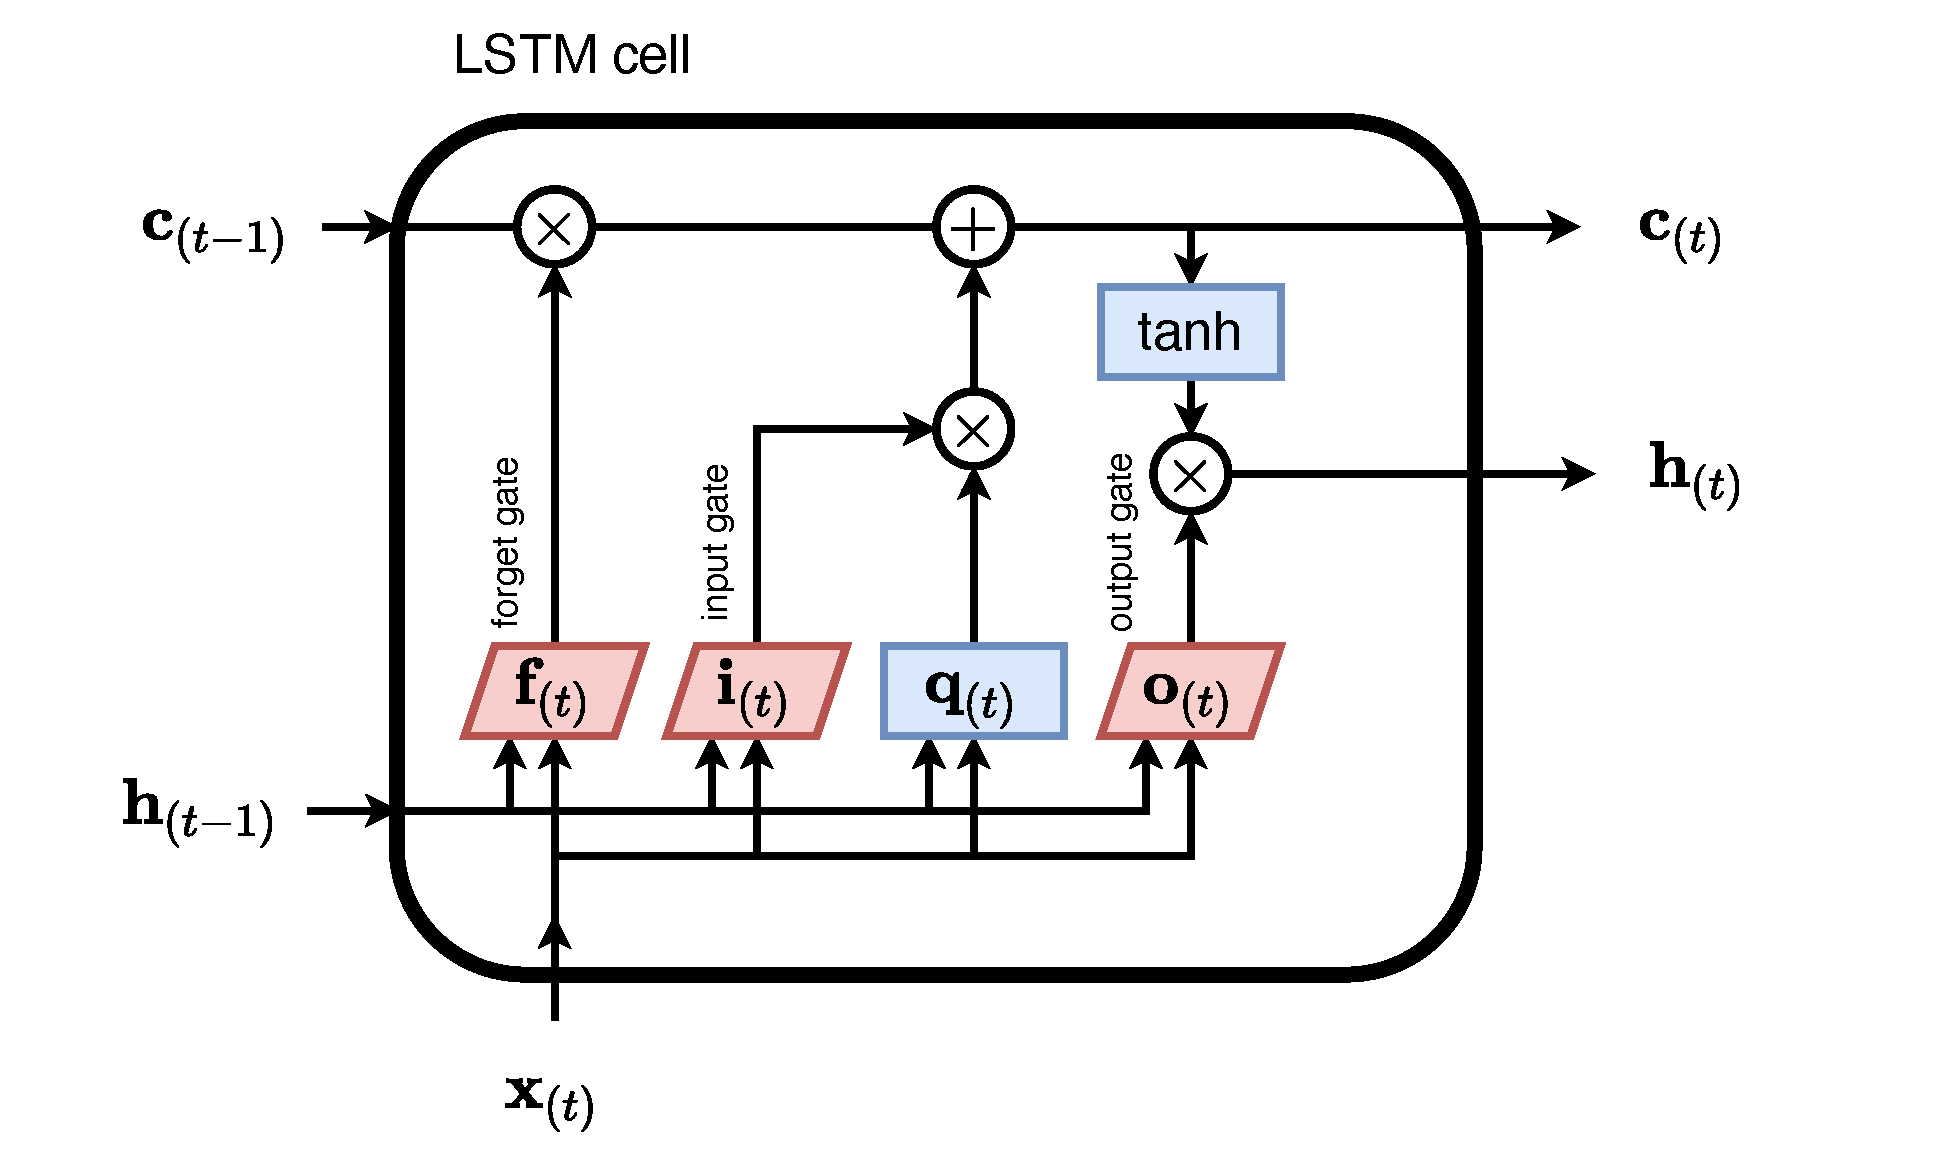
\includegraphics{./src/lstm}
\caption{\label{fig:lstmcell} Long short-term memory cell}
\end{figure}

\begin{align*}
\mathbf{i}_{(t)} &= \sigma(
    \mathbf{W}_{xi}^T \mathbf{x}_{(t)}
    + \mathbf{W}_{hi}^T\mathbf{h}_{(t-1)} + \mathbf{b}_i
) \\
\mathbf{f}_{(t)} &= \sigma(
    \mathbf{W}_{xf}^T\mathbf{x}_{(t)} + \mathbf{W}_{hf}^T
    \mathbf{h}_{(t-1)} + \mathbf{b}_f
) \\
\mathbf{o}_{(t)} &= \sigma(
    \mathbf{W}_{xo}^T \mathbf{x}_{(t)} +
    \mathbf{W}_{ho}^T\mathbf{h}_{(t-1)} + \mathbf{b}_o
) \\
\mathbf{q}_{(t)} &= tanh(
    \mathbf{W}_{xg}^T \mathbf{x}_{(t)} +
    \mathbf{W}^T_{hg}\mathbf{h}_{(t-1)} + \mathbf{b}_g
) \\
\mathbf{c}_{(t)} &= \mathbf{f}_{(t)} \otimes \mathbf{c}_{(t-1)} + 
    \mathbf{i}_{(t)}\otimes \mathbf{q}_{(t)}\\
\mathbf{y}_{(t)} &= \mathbf{h}_{(t)} = \mathbf{o}_{(t)}
\otimes tanh(\mathbf{c}_{(t)})
\end{align*}

\hypertarget{gan_model}{%
\subsection{GAN model}\label{gan_model}}

The GAN model consists of two competing neural networks called
discriminator and generator. The discriminator in this paper
will estimate the SDF weight function \(\omega(I_t, I_{t, i})\), and the generator will estimate the factor function
\(g(I_t, I_{t, i})\). Both models use an
LSTM network to extract signal from macroeconomic data and a
feed-forward network to extract signal from firm characteristic data.
The GAN architecture under section \protect\hyperlink{gan_structure}{subsection 3.5}
explains the model structure in-depth

\[
\text{Discriminator: } \omega(I_t, I_{t, i})
\text{, Generator:} g(I_t, I_{t, i}).
\]

Therefore, the GAN training procedure can be viewed as a
zero-sum game where the discriminator minimises the
pricing loss. In contrast, the generator tries to maximise the
pricing loss. Note that the functions estimated by
discriminator and generator are both time and asset
independent. Given a data size \(N\), we summarise the GAN training as the following
min-max optimisation problem with the pricing loss function
motivated by the no-arbitrage condition

\begin{align*}
    \min_{\omega} \max_{g} L(\omega, g|I_t, I_{t, i}) &=
    \frac{1}{N} \sum_{i=1}^N \left\{
    E \left[ \left( 1 - \sum_{j=1}^N \omega(I_t, I_{t, j})
    R^e_{t+1, j} \right) R^e_{t+1, j}g(I_t, I_{t, i})
    \right] \right\}^2.
\end{align*}

\hypertarget{factor-models}{%
\subsection{Factor models}\label{factor-models}}

The Carhart (1997) four-factor model builds on
Fama \& French (1993)'s three-factor model. This paper uses the
four-factor model as the benchmark against the GAN model.

The three-factor model aims
to explain the assets' excess returns through (1) market
risk (\(R^e_{mt}\)),
(2) outperformance of small market capitalisation
companies relative to large market capitalisation companies
(small minus big, SMB)
and (3) the outperformance of high book-to-market value
companies versus low book-to-market value companies (high
minus low, HML).
On the other hand, the four-factor model further included a
momentum (UMD) factor to account for the speed of price
change.
If the factor model correctly explains the variation in
asset prices, we expect a no-intercept regression with
\(E(\alpha_i)=0\).
Formally the model can be described by the following
equation, where \(R^e_{t+1, i}\) is asset i's excess return,

\[
R^e_{t+1, i} = \alpha_i + \beta_i R^e_{mt} + s_i SMB_t + h_i HML_t + \omega_i UMD_t + \epsilon_{t, i}.
\]

Therefore, in contrast to the non-linear, non-parametric GAN model,
the factor model can be considered as a
parametric model where assets' excess return is a linear
combination of the constructed factors.

\hypertarget{model_training}{%
\section{Model Training}\label{model_training}}

\thispagestyle{plain}

This chapter explains the methodology used to train the
GAN and the factor model. We first describe a
general neural network training before focusing on the GAN model.

\hypertarget{training-a-neutral-network}{%
\subsection{Training a neutral network}\label{training-a-neutral-network}}

Training a neural network is an empirical experiment.
We used Chen et al.~(2019)'s best-performing
hyper-parameters choices, including the number of hidden
units and number of hidden layers, while following the best
practice of neural network training, including dynamic
learning rate and regularization.

\hypertarget{adam}{%
\subsubsection{Adam Optimizer}\label{adam}}

As explained in the \protect\hyperlink{nn_model}{subsection 3.3}, back-propagation
is one critical component in the training procedure.
We used adaptive moment estimation (Adam) proposed by
Kingma \& Ba (2015), which combines momentum optimization and
RMSProp, another optimizer popular before Adam. We define
\(\mathbf{\theta}\) as the multi-variable weights,
\(\nabla_{\mathbf{\theta}}L(\mathbf{\theta})\) as the
multi-variable gradient with respect to a loss function \(L(\cdot)\),
\(\eta\) as the learning rate,
\(\mathbf{m}\) as the momentum vector, and \(\mathbf{s}\) as the
squared of momentum vector,
\(\beta_1\) as the momentum rate,
\(\beta_2\) as the decay rate,
\(\epsilon\) as the smoothing parameter to avoid zero
division,
\(\otimes\) as the element wise multiplication,
and \(\oslash\) as the element wise division.
In contrast to a gradient descent algorithm where the
updating rule is independent of the previous gradients:
\(\mathbf{\theta} \leftarrow \mathbf{\theta} - \eta \nabla_{\mathbf{\theta}} L(\mathbf{\theta})\),
a general momentum algorithm includes an additional parameter
\(\mathbf{m}\) that captures the value of previous gradients,
allowing for faster convergence.
Adaptive gradient methods scale down the gradient by the
past gradient value \(\sqrt{\mathbf{s}}\), decaying the steeper
gradients more than the smoother gradients, allowing the
parameter to convergence even faster.
Adam combined the momentum and adaptive gradients
techniques.

A momentum algorithm is described as:

\begin{enumerate}
\def\labelenumi{\arabic{enumi}.}
\tightlist
\item
  \(\mathbf{m} \leftarrow \beta_1 \mathbf{m} - \eta \nabla_{\mathbf{\theta}}L(\mathbf{\theta})\)
\item
  \(\mathbf{\theta}\leftarrow \mathbf{\theta} + \mathbf{m}\)
\end{enumerate}

An adaptive gradient algorithm is described as:

\begin{enumerate}
\def\labelenumi{\arabic{enumi}.}
\tightlist
\item
  \(\mathbf{s} \leftarrow \beta_2 \mathbf{s} + (1-\beta_2) \nabla_{\mathbf{\theta}} L(\mathbf{\theta}) \otimes \nabla_{\mathbf{\theta}}L(\mathbf{\theta})\)
\item
  \(\mathbf{\theta} \leftarrow \mathbf{\theta} - \eta \nabla_{\mathbf{\theta}}L(\mathbf{\theta}) \oslash \sqrt{\mathbf{s} + \epsilon}\)
\end{enumerate}

The Adam algorithm is described as:

\begin{enumerate}
\def\labelenumi{\arabic{enumi}.}
\tightlist
\item
  \(\mathbf{m} \leftarrow \beta_1 \mathbf{m} - (1-\beta_1) \nabla_{\mathbf{\theta}} L(\mathbf{\theta})\)
\item
  \(\mathbf{s} \leftarrow \beta_2 \mathbf{s} + (1-\beta_2) \nabla_{\mathbf{\theta}} L(\mathbf{\theta}) \otimes \nabla_{\mathbf{\theta}} L(\mathbf{\theta})\)
\item
  \(\hat{ \mathbf{m} } \leftarrow \frac{\mathbf{m}}{1-\beta_1^t}\)
\item
  \(\hat{ \mathbf{s} } \leftarrow \frac{\mathbf{s}}{1-\beta_2^t}\)
\item
  \(\mathbf{\theta} \leftarrow \mathbf{\theta} + \eta \hat{ \mathbf{m} } \oslash \sqrt{\hat{ \mathbf{s} } + \epsilon}\)
\end{enumerate}

\hypertarget{dynamic-learning-rate-with-learning-schedule}{%
\subsubsection{Dynamic learning rate with learning schedule}\label{dynamic-learning-rate-with-learning-schedule}}

The learning rate \(\eta\) affects the extent to which gradients are
updated by changing the step size in the gradient
descent method. A too high learning rate prevents gradient descent
from converging while a too low learning rate significantly
increases the training time. Instead of using a fixed
learning rate, this paper adopts exponential scheduling
where the learning rate is updated as the training epochs
\(t\) increase. We denote \(\eta_0\) as the initial learning
rate, \(s\) as a hyper-parameter step that decreases the
impact of the initial \(s\) training epochs. As a result, the
learning rate decreases faster as the training epochs
increase

\[
\eta(t) = \eta_0 0.1 ^{t/s}.
\]

\hypertarget{regularization}{%
\subsubsection{Regularization}\label{regularization}}

Regularization refers to techniques used to prevent
over-fitting. Over-fitting occurs when the model is tuned
solely on the training data and does not generalise well in
unseen test data. For example, LASSO and Ridge modify
least square regression by including \(\ell 1\) and \(\ell 2\)
penalties. Deep learning provides additional regularization
techniques, including the dropout and early stopping
adopted in this paper.

\hypertarget{regularization-with-dropout}{%
\paragraph{Regularization with dropout}\label{regularization-with-dropout}}

Dropout is a simple yet powerful algorithm, users set a
hyper-parameter dropout rate \(p\), and during training, \(p\)\%
of the hidden units will not be included in the gradient
calculation. Intuitively, dropout forces the neural network
to train a new but dependent model during each training
epoch, avoiding relying on the same information each time.
Dropout is not used during prediction.

\hypertarget{regularization-with-early-stopping}{%
\paragraph{Regularization with early stopping}\label{regularization-with-early-stopping}}

Early stopping is a technique that stops model training
before the model over-fits the training data. Stopping
criteria is pre-set by the users, and for a standard neural
network, the decrease in loss function is often used as the
criteria. For example, training stops if the decrease in loss between \(t\)
and \(t+1\) is less than \(\epsilon\). However, it is
harder to decide on stopping criteria for GAN models, and
this paper uses the Sharpe ratio as the stopping criteria.

\hypertarget{gan_structure}{%
\subsection{GAN architecture}\label{gan_structure}}

As explained in \protect\hyperlink{GAN_model}{subsection 3.5}, a GAN model
alternates between training a discriminator and generator.
To further increase the convergence speed,
we first train the individual network separately in a
standard neural network training procedure before training
them in a GAN framework.

\hypertarget{discriminator-network-structure}{%
\subsubsection{Discriminator network structure}\label{discriminator-network-structure}}

As illustrated in Figure \ref{fig:discriminator}, the discriminator network has
two input layers, one for macroeconomic data and another
for firm characteristics data. The network concatenates the
latent variables produced by the LSTM layer
and firm characteristics to produce a single output
corresponding to the stochastic discount factor (SDF) weight
\(\mathbf{\omega_t}\). Therefore, the training for discriminator
can be expressed as the following equation

\[
\min_{\omega} L(\omega|\hat{g}, I_t, I_{t,i}).
\]

\begin{figure}
\centering
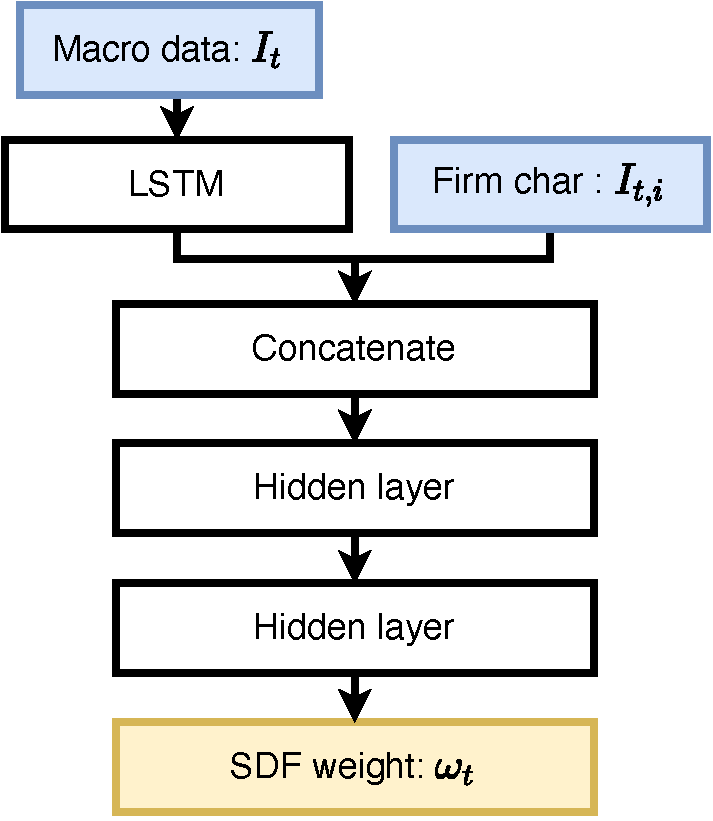
\includegraphics[width=0.4\textwidth,height=\textheight]{./src/discriminator}
\caption{\label{fig:discriminator}Discriminator structure}
\end{figure}

\hypertarget{generator-network-structure}{%
\subsubsection{Generator network structure}\label{generator-network-structure}}

As illustrated in Figure \ref{fig:generator}, the generator network shares
a similar structure as the discriminator network.
The only difference is in the output layer, where the generator
network will select factors representing a
combination of assets and firm characteristics unexplained by
the no-arbitrage condition. Therefore, the
generator training can be expressed as the following equation

\[
\max_{g} L(g|\hat\omega, I_t, I_{t,i}).
\]

\begin{figure}
\centering
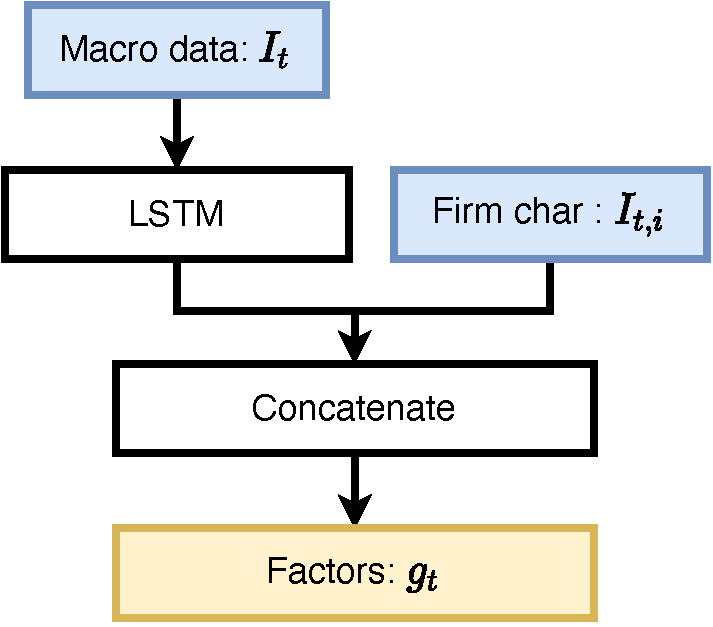
\includegraphics[width=0.4\textwidth,height=\textheight]{./src/generator}
\caption{\label{fig:generator}Generator structure}
\end{figure}

\newpage

\hypertarget{gan-network-structure}{%
\subsubsection{GAN network structure}\label{gan-network-structure}}

As shown in Figure \ref{fig:ganDiagram}, the discriminator and generator
are linked by a single pricing loss function. Discriminator
aims to decrease the pricing loss while generator seeks to
increase the pricing loss. Note that we require the SDF
weights multiplied by the excess returns before the pricing
loss calculation in constructing the SDF.

\begin{figure}
\centering
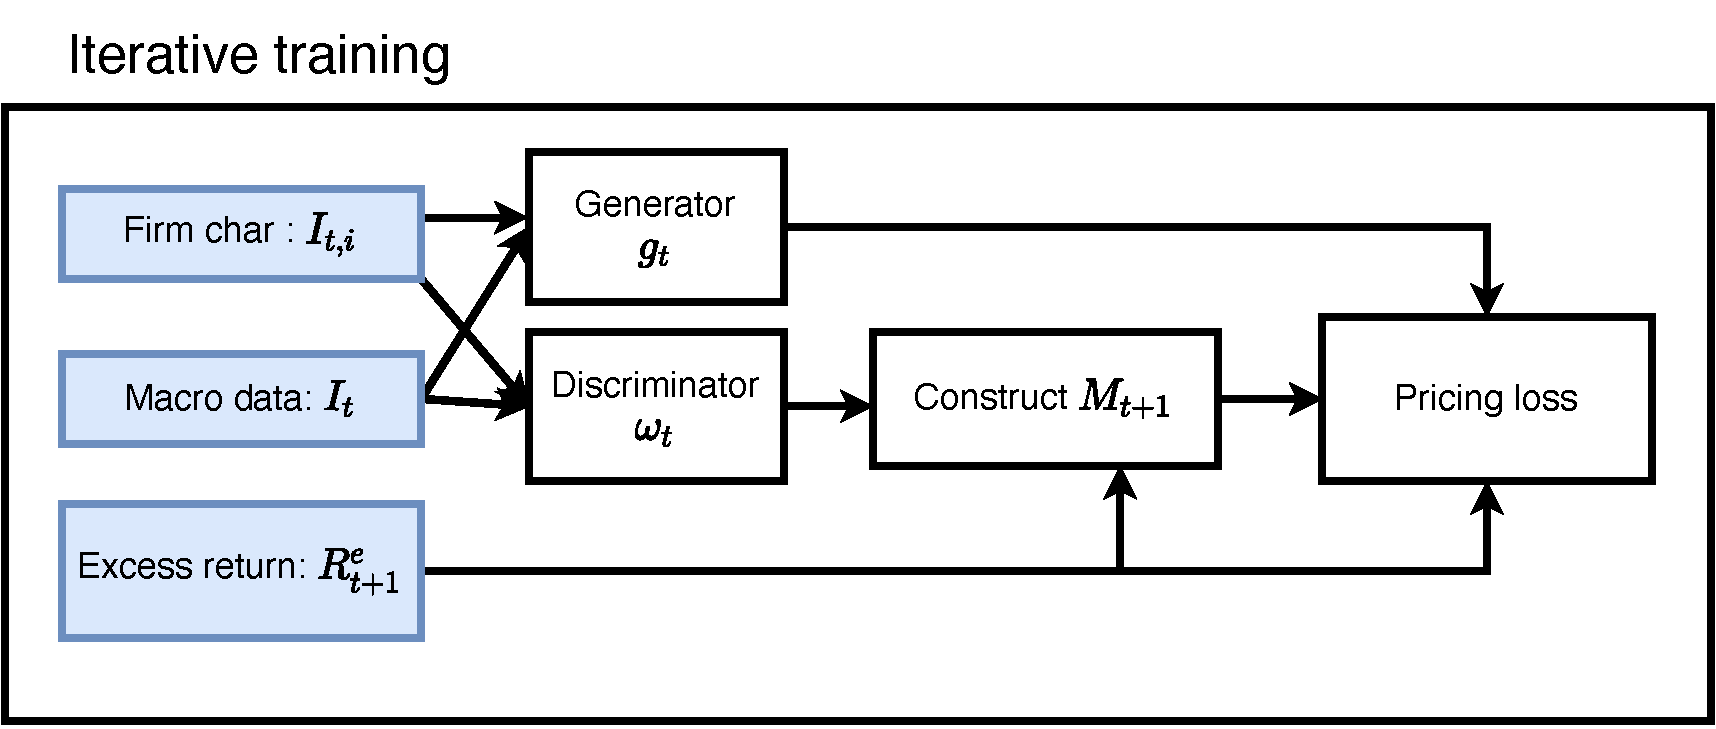
\includegraphics[width=0.7\textwidth,height=\textheight]{./src/model}
\caption{\label{fig:ganDiagram} GAN model structure}
\end{figure}

\hypertarget{empirical-no-arbitrage-asset-pricing-loss}{%
\subsubsection{Empirical no arbitrage asset pricing loss}\label{empirical-no-arbitrage-asset-pricing-loss}}

As the firms exist for different
duration, to incorporate unbalanced data, we weighted the
pricing loss to the number of non-missing data
\(T_i\)

\begin{align*}
\min_{\omega} \max_{g} L(\omega, g|I_t, I_{t, i}) &=
\frac{1}{N} \sum_{i=1}^N 
\frac{T_i}{T}
\left[ 
\frac{1}{T_i}
\sum_{t\in T_i}
\left( 1 - \sum_{j=1}^N \omega(I_t, I_{t, j}) R^e_{t+1, j} \right)
R^e_{t+1, i}g(I_t, I_{t, i})
\right]^2.
\end{align*}

\hypertarget{training-the-factor-model}{%
\subsection{Training the factor model}\label{training-the-factor-model}}

The factor model can be trained using least squares
estimation. This paper uses ordinary least squares method
for estimation.

\hypertarget{evaluation-metrics}{%
\section{Evaluation metrics}\label{evaluation-metrics}}

\thispagestyle{plain}

This paper evaluates the performance of the GAN model against the
four-factor model based on the Sharpe ratio.

\hypertarget{sharpe_ratio}{%
\subsection{Sharpe ratio}\label{sharpe_ratio}}

William F. Sharpe (1966) proposed the Sharpe ratio to evaluate
the performance of risk-adjusted assets relative to a
risk-free asset. A Sharpe ratio (\(S\))
for an asset \(i\) is defined as the asset's historical excess
return \(E_t(R^e_{i})\) weighted by the risk of the asset,
where the standard deviation of the excess return \(\sigma_i\)
approximates the risk of an asset. The excess return is the
difference between the asset's return and the risk-free
return \(E_t(R^e_{i}) = E_t(R_{i} - R^f)\). Sharpe ratio
measures the reward investors get when investing in the
asset while considering the risk of the
assets. Therefore, a higher Sharpe ratio implies the asset
is better, and the tangency portfolio \(F_{t+1}\) that lies
on the mean-variance frontier will have the highest Sharpe
ratio possible.
We compare the Sharpe ratio of the tangency portfolio by
both GAN and four-factor models to decide on the model with
better performance

\[
S(R_i) = \frac{E_t[R_i - R^f]}{\sigma_i}.
\]

\hypertarget{gan-sharpe-ratio-computation}{%
\subsubsection{GAN Sharpe ratio computation}\label{gan-sharpe-ratio-computation}}

The discriminant network in the GAN model estimates the SDF
weight \(\omega_t\). Therefore, by construction, the
tangency portfolio \(F_{t+1}\) will be defined as the dot
product between the SDF weight and assets' excess returns
\(R^e_{t+1}\) as described in the equation

\[
F_{t+1} = \omega_t^TR^e_{t+1}.
\]

\hypertarget{factor-model-sharpe-ratio-computation}{%
\subsubsection{Factor model Sharpe ratio computation}\label{factor-model-sharpe-ratio-computation}}

Let \(\omega\) be the optimal portfolio weight for factor
models, \(f\) be the factors, \(\Sigma\) be the covariance
matrix between factors and \(R^f\) be the risk free rate.
Then we can solve Sharpe ratio explicitly through the
following maximisation problem

\[
\max_{\omega} \frac{E(\omega^Tf-R^f)}{\sqrt{\omega^T\Sigma\omega}}.
\]

The optimal weight \(\omega^*\) is the solution to the
maximisation problem, which is

\[
w^* = \Sigma^{-1}E(f).
\]

The optimal Sharpe ratio \(S^*\) is then the value function

\[
S^* = \sqrt{E(f)^T\Sigma^{-1}E(f)}.
\]

\hypertarget{data}{%
\section{Data}\label{data}}

\thispagestyle{plain}

This paper extracts January 1998 to December 2017 London
Stock Exchange (LSE) monthly stock prices from Yahoo! Finance and
splits the complete data into twelve years of
training data (1998 - 2009), four years of validation data (2010 - 2013) and
four years of out-of-sample testing data (2014 - 2017).
Gregory et al. (2011) provide the risk-free rate used
to calculate excess returns, and
the monthly factor data containing small minus big
(SMB), high minus low (HML), momentum (UMD) factors and
value-weighted market portfolio returns.
Gregory et al. (2011) provide a detailed explanation for
the factor construction in their paper.
In addition to the price data, this paper also extracts sixteen
firm income statement data from \emph{Finage {LTD}} (2022),
a financial data
provider which retrieves income
statements through company reports. The income statements
follow standard accounting naming convention.
This paper interpolated quarterly income statement data into
monthly data and transformed level data using log
differences.

The analysis in this paper follows Chen et al. (2021) to remove
stocks without complete characteristics data
in a particular month.
However, the Finage database only contains limited
income statement data for a subset of stocks.
Therefore, we perform two different data splits to
maximise the data available for training.
The first dataset contains factor data and past returns data
for 942 stocks.
The second dataset used for training includes factor data, past returns and
income statement data which accounts for 242 stocks.
Furthermore, we refer to the dataset based on only
factor and past returns as \emph{factor data} while the
dataset based on the factor, past returns and income
statement data as \emph{fundamental data}.
Table \ref{tab:firm-data} summarises the training data.

Additionally, we retrieve a large macroeconomic dataset from
Coulombe et al. (2021).
The dataset contains 112 monthly
macroeconomic indicators comprising of
nine categories from domestic productions to price index,
international trade and interest rates.
Coulombe et al. (2021) have transformed the macroeconomic data into
stationary time series, so this paper does not require any further data
processing.
Their paper and \href{https://www.stevanovic.uqam.ca/DS_UKMD.html}{website}
contain detailed information on data construction and
handling.

\blandscape

\begin{longtable}[]{@{}
  >{\centering\arraybackslash}p{(\columnwidth - 8\tabcolsep) * \real{0.1468}}
  >{\raggedright\arraybackslash}p{(\columnwidth - 8\tabcolsep) * \real{0.5183}}
  >{\centering\arraybackslash}p{(\columnwidth - 8\tabcolsep) * \real{0.0642}}
  >{\centering\arraybackslash}p{(\columnwidth - 8\tabcolsep) * \real{0.0872}}
  >{\centering\arraybackslash}p{(\columnwidth - 8\tabcolsep) * \real{0.1835}}@{}}
\caption{\label{tab:firm-data} Firm-specific Training data}\tabularnewline
\toprule
\begin{minipage}[b]{\linewidth}\centering
Characteristics
\end{minipage} & \begin{minipage}[b]{\linewidth}\raggedright
Description
\end{minipage} & \begin{minipage}[b]{\linewidth}\centering
Factor data
\end{minipage} & \begin{minipage}[b]{\linewidth}\centering
Fundamental data
\end{minipage} & \begin{minipage}[b]{\linewidth}\centering
Data Source
\end{minipage} \\
\midrule
\endfirsthead
\toprule
\begin{minipage}[b]{\linewidth}\centering
Characteristics
\end{minipage} & \begin{minipage}[b]{\linewidth}\raggedright
Description
\end{minipage} & \begin{minipage}[b]{\linewidth}\centering
Factor data
\end{minipage} & \begin{minipage}[b]{\linewidth}\centering
Fundamental data
\end{minipage} & \begin{minipage}[b]{\linewidth}\centering
Data Source
\end{minipage} \\
\midrule
\endhead
excess returns & Return of an asset minus risk free rate & Y & Y & Yahoo! Finance, Gregory et al.~(2011) \\
rmrf & Excess return for market portfolio, market risk premium factor & Y & Y & Gregory et al.~(2011) \\
hml & High minus Low, value factor & Y & Y & Gregory et al.~(2011) \\
smb & Small minus Big, size factor & Y & Y & Gregory et al.~(2011) \\
umd & Momentum & Y & Y & Gregory et al.~(2011) \\
r2\_1 & Short-term momentum, computed as lagged one-month return & Y & Y & Yahoo! Finance \\
r12\_7 & Intermediate momentum, cumulative return from 12 to 7 months before the return prediction & Y & Y & Yahoo! Finance \\
cost and expenses & Cost and expense & N & Y & Finage \\
depreciation and amortization & Depreciation and Amortization & N & Y & Finage \\
ebitda & Earnings Before Interest, Taxes, Depreciation, and Amortization & N & Y & Finage \\
ebitdaratio & EBITDA to sales ratio & N & Y & Finage \\
eps & Earnings per share & N & Y & Finage \\
epsdiluted & Diluted Earnings per Share & N & Y & Finage \\
income before tax & Earnings before tax & N & Y & Finage \\
income before taxRatio & Pretax profit margin & N & Y & Finage \\
netincome & Net income, the amount an individual or business makes after deducting costs, allowances and taxes & N & Y & Finage \\
netincomeratio & Net profit margin & N & Y & Finage \\
operatingincome & Amount of profit generated from a business operation, after deducing operating expenses & N & Y & Finage \\
revenue & Revenue, sales generated from business operations & N & Y & Finage \\
weighted averageshsout & Weighted average of outstanding shares & N & Y & Finage \\
weighted averageshsout dil & Diluted weighted average of outstanding shares & N & Y & Finage \\
\bottomrule
\end{longtable}

\elandscape

\hypertarget{empirical-findings}{%
\section{Empirical findings}\label{empirical-findings}}

\thispagestyle{plain}

The \protect\hyperlink{data}{Data} section describes two types of
datasets: \emph{factor} and \emph{fundamental} data.
The \emph{factor data} training contains more assets but lesser
characteristic data, while \emph{fundamental data} training
contains more characteristic data with lesser assets.
Therefore, readers should consider differences across the
datasets used when interpreting the results.
Generally, neural network models require a large dataset for
training. However, as \emph{Google {LLC}} (2019) recommended in their
developer website, there is no common consensus among
literature and the required size of dataset may be
context-dependent.

\hypertarget{sharpe-ratio}{%
\subsection{Sharpe ratio}\label{sharpe-ratio}}

GAN models generally achieve a higher out-of-sample Sharpe
ratio than the four-factor model. The GAN model trained on
factor and macroeconomic data has achieved the highest Sharpe
ratio of 1.99 in the test period compared to 0.42 in
the four-factor model.
However, the GAN model trained solely on factor data has achieved a
Sharpe ratio of 0.33, which was lower than the four-factor model.
Meanwhile, the GAN models trained on fundamental data achieve a higher
out-of-sample Sharpe ratio at 0.49 (without macroeconomic
data) and 0.69 (with macroeconomic data) than the
four-factor models.
Therefore, the overall trend in the results shows that the GAN models
outperform the four-factor model, which is consistent with
Chen et al. (2021)'s finding.

Additionally, this paper finds that adding macroeconomic data
can improve the GAN models in both datasets. The Sharpe ratio of
GAN models trained on macroeconomic factors outperformed the
GAN models trained on the same dataset, without
macroeconomic data. The improvement in
model performance suggests that macroeconomic data
has a role in estimating the SDF, which aligns with
Chen et al. (2021)'s finding.

However, the Sharpe ratio is lower than the GAN model
trained without the additional fundamental data.
Although fundamental data was relevant in Chen et al. (2021)'s
paper, the GAN models trained with income
statement data do not outperform those trained without
income statement data in this paper.
The two possible reasons for the lower performance could be
either the irrelevance of income statement data or the
narrower range of fundamental data available for the UK.
In our results, the GAN model trained solely on fundamental data
outperformed the GAN model trained solely on factor
data. Therefore, this paper suggests that the lower
performance could be due to the smaller dataset.
As mentioned earlier, fundamental sample contains 242 stocks, while the factor
sample contains 942 stocks. Since all GAN models have the
same parameter setting, there could be insufficient data for
GAN models trained with fundamental data, and income
statements could still be relevant in estimating the SDF.

In contrast to Chen et al. (2021)'s result, the Sharpe ratios
in this paper do not decrease sharply from the in-sample
period to the out-of-sample period.
Chen et al. (2021) achieved a Sharpe ratio of 2.68 in the
training period, 1.43 in the validation period and 0.75 in
the testing period. However, the best performing GAN model in this
paper achieved a Sharpe ratio of 1.88 in the training
period, 1.76 in the validation period and even higher Sharpe
ratio of 1.99 in the testing period. Even the factor model
achieve a higher Sharpe ratio of 0.42 in the testing period than the
Sharpe ratio of 0.29 in the training period.
The stable Sharpe ratio suggests that although we expect the
SDF functional form to be time-varying, the UK SDF
functional form might be relatively consistent across the 5
to 10 year period.
Table \ref{tab:sharpe-result} summarises the Sharpe ratio
for different models.

\begin{longtable}[]{@{}
  >{\centering\arraybackslash}p{(\columnwidth - 10\tabcolsep) * \real{0.1250}}
  >{\centering\arraybackslash}p{(\columnwidth - 10\tabcolsep) * \real{0.1944}}
  >{\centering\arraybackslash}p{(\columnwidth - 10\tabcolsep) * \real{0.3056}}
  >{\centering\arraybackslash}p{(\columnwidth - 10\tabcolsep) * \real{0.1111}}
  >{\centering\arraybackslash}p{(\columnwidth - 10\tabcolsep) * \real{0.1111}}
  >{\centering\arraybackslash}p{(\columnwidth - 10\tabcolsep) * \real{0.1111}}@{}}
\caption{\label{tab:sharpe-result} Sharpe ratio results}\tabularnewline
\toprule
\begin{minipage}[b]{\linewidth}\centering
Model
\end{minipage} & \begin{minipage}[b]{\linewidth}\centering
Data used
\end{minipage} & \begin{minipage}[b]{\linewidth}\centering
Included Macro data
\end{minipage} & \begin{minipage}[b]{\linewidth}\centering
Train
\end{minipage} & \begin{minipage}[b]{\linewidth}\centering
Valid
\end{minipage} & \begin{minipage}[b]{\linewidth}\centering
Test
\end{minipage} \\
\midrule
\endfirsthead
\toprule
\begin{minipage}[b]{\linewidth}\centering
Model
\end{minipage} & \begin{minipage}[b]{\linewidth}\centering
Data used
\end{minipage} & \begin{minipage}[b]{\linewidth}\centering
Included Macro data
\end{minipage} & \begin{minipage}[b]{\linewidth}\centering
Train
\end{minipage} & \begin{minipage}[b]{\linewidth}\centering
Valid
\end{minipage} & \begin{minipage}[b]{\linewidth}\centering
Test
\end{minipage} \\
\midrule
\endhead
Factor & factor & N & 0.29 & 0.62 & 0.42 \\
GAN & factor & N & 0.65 & 0.49 & 0.33 \\
GAN & factor & Y & 1.88 & 1.76 & 1.99 \\
GAN & fundamental & N & 0.70 & 0.35 & 0.49 \\
GAN & fundamental & Y & 1.18 & 0.39 & 0.69 \\
\bottomrule
\end{longtable}

\newpage

\hypertarget{variable-importance}{%
\subsection{Variable importance}\label{variable-importance}}

To better understand how each variable affects the SDF
weight, we have computed sensitivity score following
Chen et al. (2021)'s paper. The sensitivity score measures the
change in SDF weight \(\omega\) as a variable changes. Mathematically, this
is the average absolute gradient expressed in the following
equation. We define \(C\) normalising constant scaling
sensitivity scores between 0 and 1. A higher
sensitivity means the variable has a larger effect on the
SDF weight \(\omega\) with 0 being not relevant and 1 being
the most important variable.

\[
\text{Sensitivity}(x_j) = \frac{1}{C} \sum_{i=1}^N \sum_{t=1}^T
    \left|  \frac{\partial \omega(I_t, I_{t, i})}{\partial x_j} \right|.
\]

In this paper, we focus our analysis on the top performing model: the GAN
trained on factor and macroeconomic data.
With reference to Figure \ref{fig:vi}, the top four most
important variables are the four factors in the factor
model (RMRF, HML, UMD, SMB). This thus suggests that the
factors are indeed very crucial in estimating the SDF weight.
Following the factors, we have the two firm
specific past return data and this implies that the firm specific
characteristics are important as well. For macroeconomic
data, we notice that the top ten macroeconomic data
contributed the most to the SDF weight. The top ten
macroeconomic data revolve around indexes affecting
consumers, business and the general stock markets. The top
ten macroeconomic data include producer price indices (PPI) of
different UK domestic markets, Composite leading indicator (CLI),
Consumer and Business confidence index (CCI, BCI)
iShares MSCI United Kindom ETF (UK\_focused\_equity) which
tracks the mid and large size companies in UK market,
and Standard \& Poor 500 (SP500).
Interestingly, the UK SDF weight is also affected by the US
market, suggesting the possible benefits of including more US
market data in future studies.

\begin{figure}
\centering
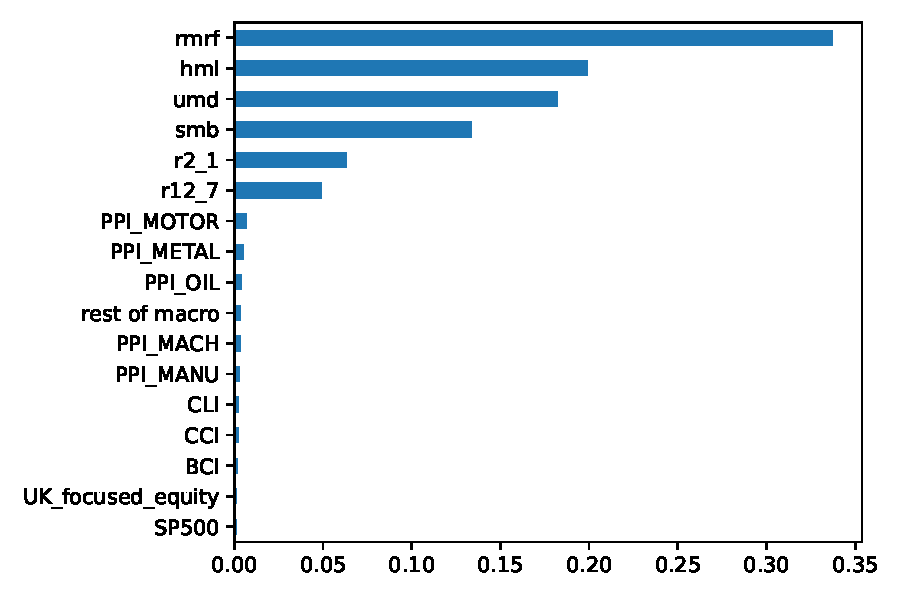
\includegraphics[width=0.6\textwidth,height=\textheight]{./src/vi}
\caption{\label{fig:vi} Variable importance}
\end{figure}

\newpage

\hypertarget{sdf-structure}{%
\subsection{SDF structure}\label{sdf-structure}}

We also studied the SDF weight structure as a function of the
factors and discovered the same two observations in
Chen et al. (2021)'s paper.
Firstly, factors in the four factor model have a linear relationship
with the SDF weight.
Secondly, there is an interaction
between these factors.
Figure \ref{fig:structure} plots the different combinations
of factors in a matrix form. The order of row and columns
represents value factor (HML), market excess return (RMRF),
size factor (SMB), momentum (UMD). The figure is achieved by
keeping all other factors at the mean level while changing
one of the factors.
The diagonal entries
show the general relationship between the factors and the SDF
weight. Moreover, the off-diagonal entries illustrate the
interaction effects between factors.
The different coloured lines correspond to different values of the
respective factors.
Upon analysis, all factors at the diagonal entries have a near
linear relationship with the SDF weight. This explains why
linear factor models generally work well.
On the other hand, we observe a
non-trivial interaction effects between the factors at the
off-diagonal entries.
Therefore, non-linear models such as the GAN model which
takes into account in the interactions between the factors
are able to perform better than linear models.

\newpage

\begin{figure}
\centering
\begin{picture}(1000, 500)
\put(0, 0){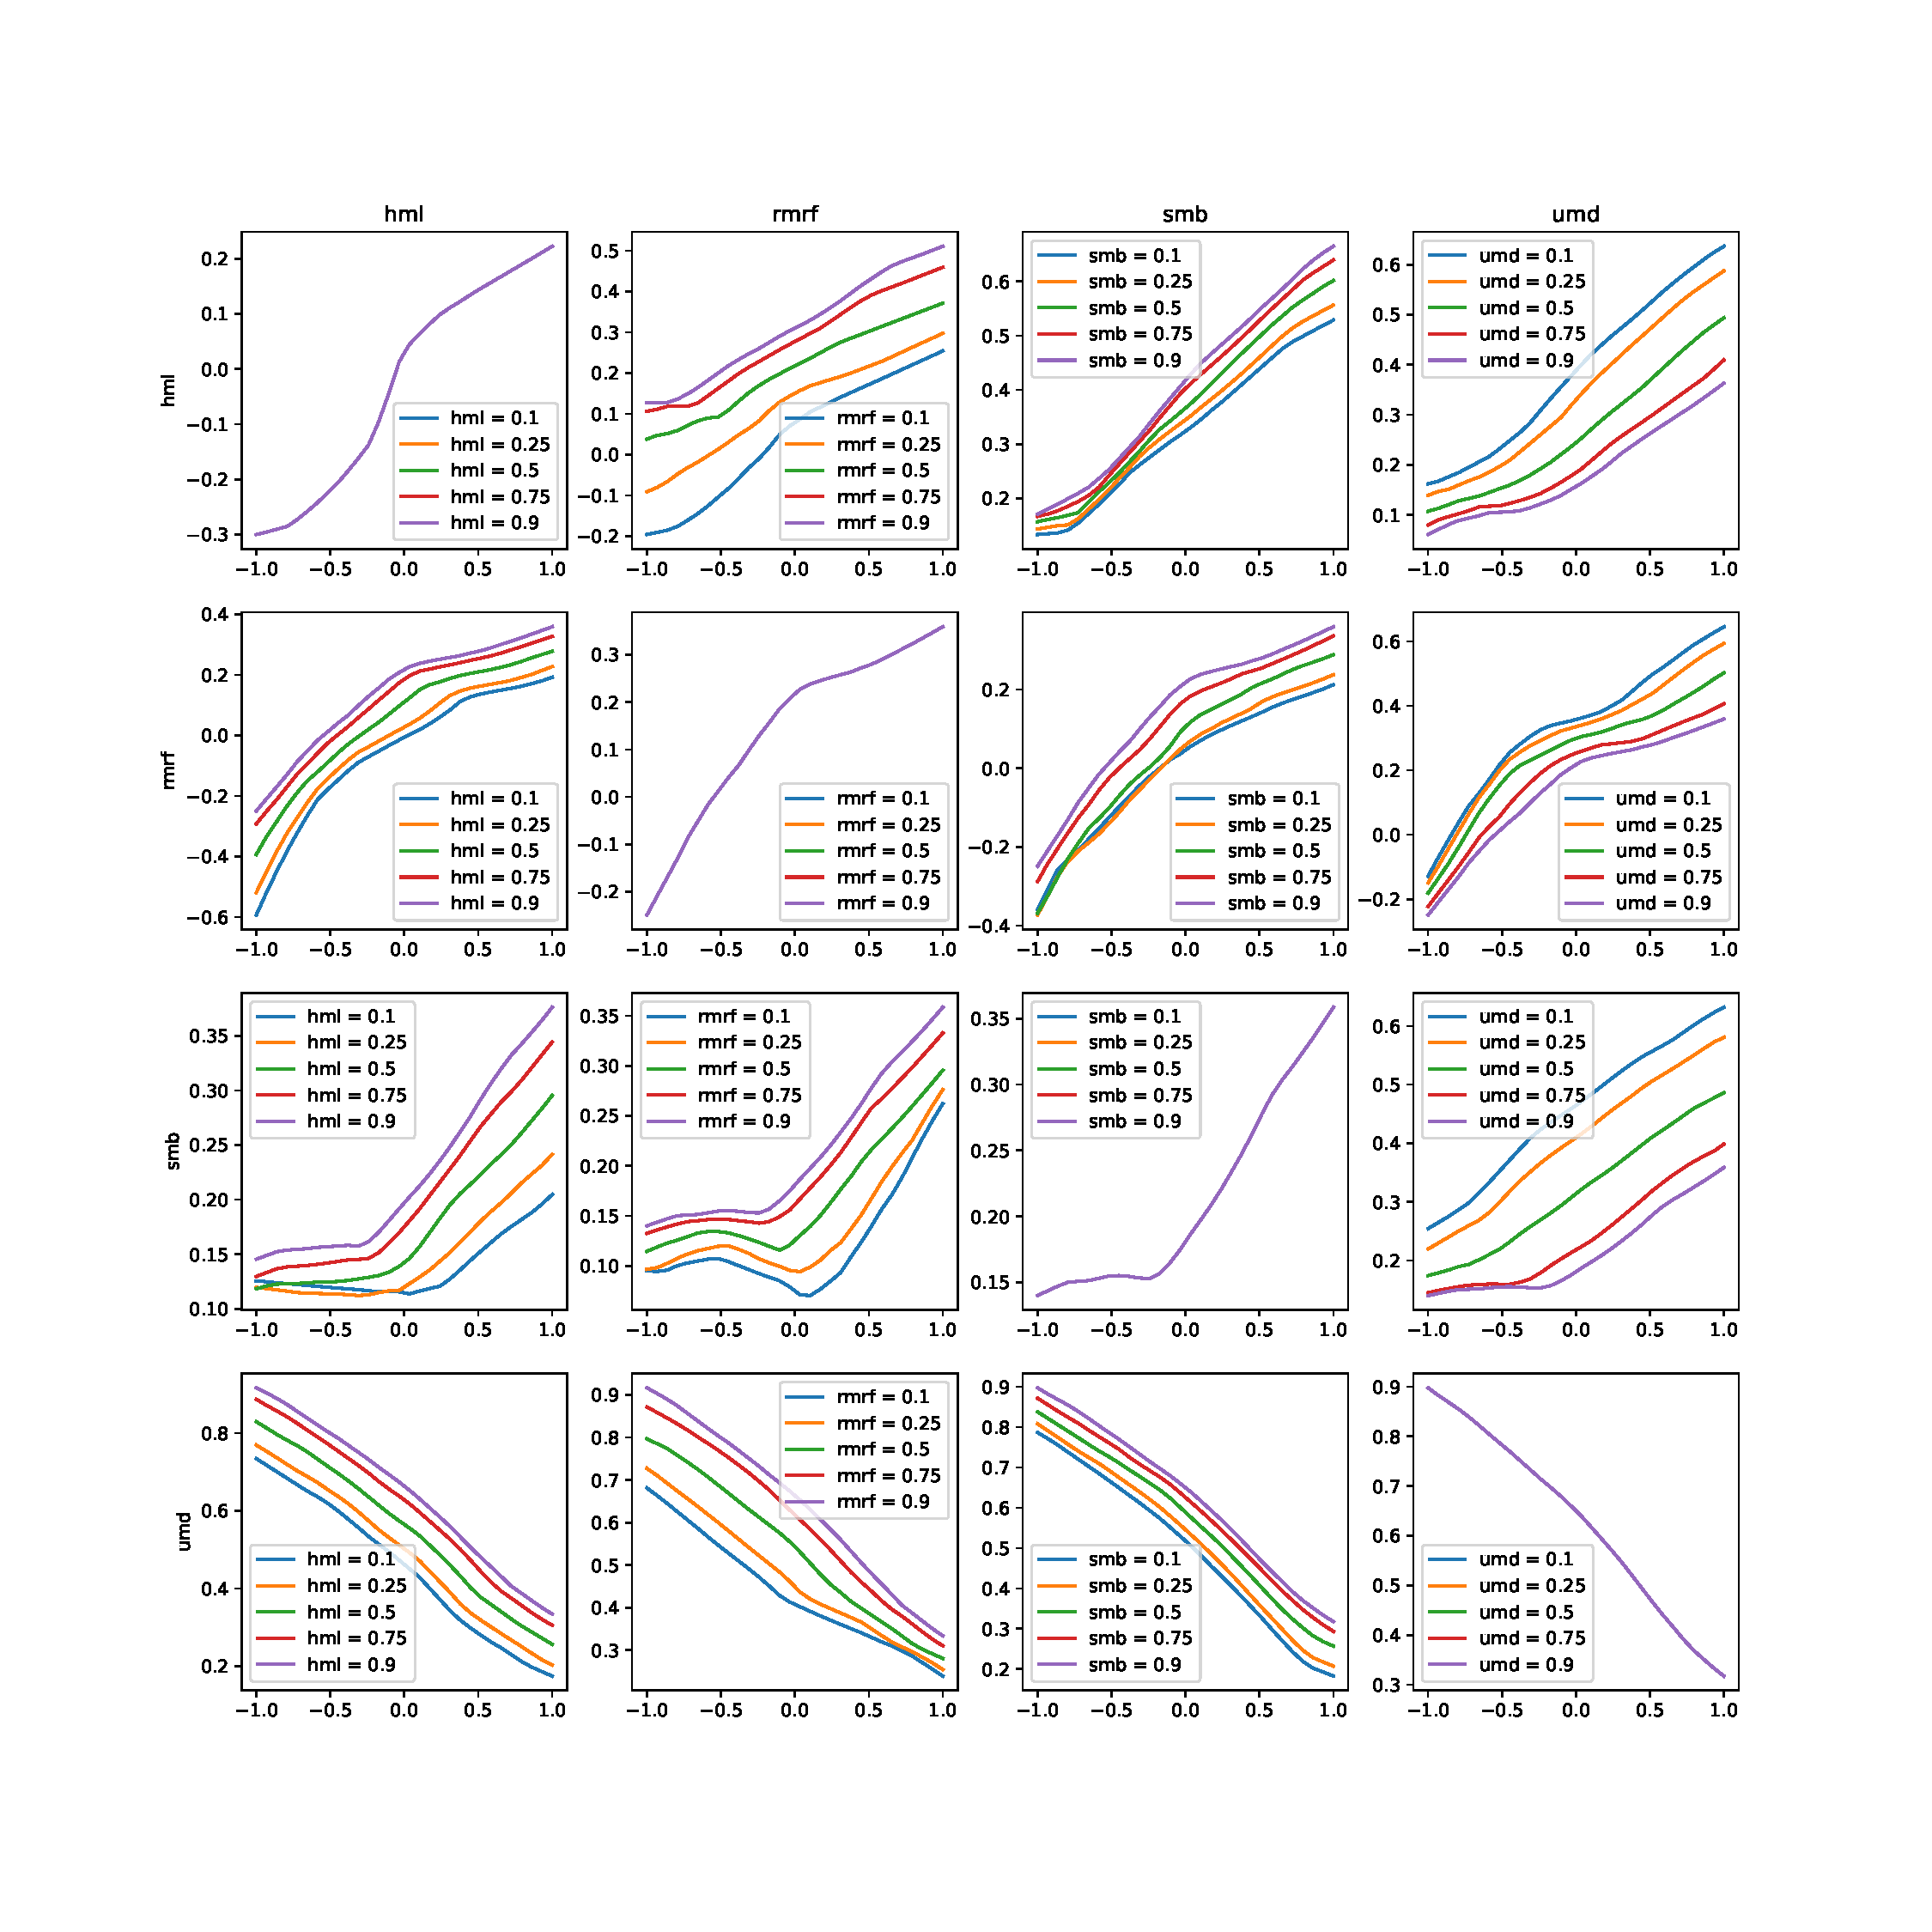
\includegraphics[width=1.1\textwidth,height=\textheight]{./src/interaction}}
\put(50, 20){The different coloured lines correspond to different values of the
respective factors}
\end{picture}
\caption{\label{fig:structure} GAN SDF weight as a function of factors}
\end{figure}

\newpage

\newpage

\hypertarget{discussion}{%
\section{Discussion}\label{discussion}}

\thispagestyle{plain}

This paper empirically validates Chen et al. (2021)'s GAN
model using UK data. However, the smaller dataset used in this paper
poses a challenge to the empirical approach. Furthermore,
this paper lacks discussion on the affordability and
environmental impact of neural network training.

Firstly, despite the effort of this paper to maximise the
data available, there is a considerable gap between the dataset
from Chen et al. (2021)'s paper and ours.
Chen et al. (2021) data include 50 years of historical data
with over 10,000 stocks. Although the number of
macroeconomic data available is comparable (178 in
Chen et al. (2021)'s paper and 112 in this paper), the number
of firm characteristics data available and the number of
stocks available are limited.
As Karras et al. (2020) and Zhao et al. (2020)
pointed out, training GAN models
with little data generally leads to the discriminator network
over-fitting the training data.
However, proposed solutions in the current literature are
only applicable to image data and is not applicable to this
paper.
The data-poor nature of the U.K. market could be one
of the crucial factors resulting in most of the literature
focusing on the U.S data, as mentioned in our literature
review.
Even the paid subscription provider was not able to
furnish complete and rich data comparable to the US.
Therefore, the results in this paper are still
relevant in assessing the performance of the GAN model when
subject to data limitations.

Secondly, this paper did not mention the affordability and
environmental impact of using the GAN model. Neural network
models such as the GAN model require Graphics Processing
Unit (GPU). GPU is a specialised electronic circuit
initially built for the gaming industry and later adopted to
neural network training due to the multiple simultaneous
computations available.
Entry-level GPU used in this paper costs a
few hundred USD while the GPU used in Chen et al. (2021)'s
costs over three thousand USD, according to the price listed
in the GPU supplier \emph{Nvidia Corporation} (2022). Moreover,
Chen et al. (2021) used eight such GPUs for the model training. Training
neural networks is also an energy-intensive task, and
Strubell et al. (2019) show that the literature seldom discuss
the high carbon emissions produced by training complicated models.

\hypertarget{conclusion}{%
\section{Conclusion}\label{conclusion}}

\thispagestyle{plain}

In conclusion, this paper delivers four key findings.
Firstly, this paper found that Chen et al. (2021)'s GAN model
is applicable to the U.K. market, where the model outperformed the
benchmark of four-factor model in terms of Sharpe ratio.
The Sharpe ratio of the GAN models trained on all datasets
is higher than the four-factor model, except the GAN
model trained only on past return data.
Secondly, similar to Chen et al. (2021)'s finding,
macroeconomic data is essential in estimating the SDF functional
form.
The GAN models estimated with macroeconomic data have a
higher Sharpe ratio than the GAN models estimated
without macroeconomic data, and the best performing
GAN model requires macroeconomic data.
Lastly,
the Sharpe ratio in the training period is comparable to the
out-of-sample test period, suggesting that the U.K. SDF
functional form seems to be consistent over time.
Having said that, the consistency applies to the period
explored in this paper. It is uncertain if the SDF will remain
consistent after Brexit or COVID-19.
This paper empirically showed that the factors relevant in
estimating the SDF. Furthermore, factors are linear in the
SDF, providing justifications for linear factor models.
However, there is an interaction effect between the factors
and models like the GAN which considers such interaction effect
would likely outperforms linear models.
With reference to the U.K. LSE 1998 - 2017 data,
this paper concludes that considering the GAN model does
value added to the empirical asset pricing.

\newpage

\hypertarget{bibliography}{%
\section{Bibliography}\label{bibliography}}

\thispagestyle{plain}

\hypertarget{refs}{}
\begin{CSLReferences}{1}{0}
\leavevmode\vadjust pre{\hypertarget{ref-bhatnagar_capital_2012}{}}%
Bhatnagar, C. S., \& Ramlogan, R. (2012). The capital asset pricing model versus the three factor model: A united kingdom perspective. \emph{International Journal of Business and Social Research}, \emph{2}, 51--65.

\leavevmode\vadjust pre{\hypertarget{ref-campbell_explaining_2000}{}}%
Campbell, J. Y., \& Cochrane, J. H. (2000). Explaining the poor performance of consumption-based asset pricing models. \emph{The Journal of Finance}, \emph{55}(6), 2863--2878. \url{http://www.jstor.org/stable/222404}

\leavevmode\vadjust pre{\hypertarget{ref-carhart_persistence_1997}{}}%
Carhart, M. M. (1997). On persistence in mutual fund performance. \emph{Journal of Finance}, \emph{52}, 57--82. \url{https://doi.org/10.2307/2329556}

\leavevmode\vadjust pre{\hypertarget{ref-chen_deep_2021}{}}%
Chen, L., Pelger, M., \& Zhu, J. (2021). Deep learning in asset pricing. \emph{Research Methods \& Methodology in Accounting {eJournal}}. \url{https://doi.org/10.2139/ssrn.3350138}

\leavevmode\vadjust pre{\hypertarget{ref-coulombe_can_2021}{}}%
Coulombe, P. G., Marcellino, M., \& Stevanović, D. (2021). Can machine learning catch the {COVID}-19 recession? \emph{{SSRN} Electronic Journal}. \url{https://doi.org/10.2139/ssrn.3796421}

\leavevmode\vadjust pre{\hypertarget{ref-fama_common_1993}{}}%
Fama, E. F., \& French, K. R. (1993). Common risk factors in the returns on stocks and bonds. \emph{Journal of Financial Economics}, \emph{33}, 3--56. \url{https://doi.org/10.1016/0304-405X(93)90023-5}

\leavevmode\vadjust pre{\hypertarget{ref-fama_five-factor_2015}{}}%
Fama, E. F., \& French, K. R. (2015). A five-factor asset pricing model. \emph{Journal of Financial Economics}, \emph{116}(1), 1--22. \url{https://doi.org/10.1016/j.jfineco.2014.10.010}

\leavevmode\vadjust pre{\hypertarget{ref-feng_taming_2020}{}}%
Feng, G., Giglio, S., \& Xiu, D. (2020). Taming the factor zoo: A test of new factors. \emph{The Journal of Finance}, \emph{75}(3), 1327--1370. \url{https://doi.org/10.1111/jofi.12883}

\leavevmode\vadjust pre{\hypertarget{ref-noauthor_finage_2022}{}}%
\emph{Finage {LTD}. Finage {\textbar} real-time stock {APIs} and websocket}. (2022). \url{https://finage.co.uk/}

\leavevmode\vadjust pre{\hypertarget{ref-freyberger_dissecting_2017}{}}%
Freyberger, J., Neuhierl, A., \& Weber, M. (2017). Dissecting characteristics nonparametrically. \emph{{CESifo}: Macro}. \url{https://doi.org/10.3386/w23227}

\leavevmode\vadjust pre{\hypertarget{ref-geron_hands-machine_2017}{}}%
Géron, A. (2017). \emph{Hands-on machine learning with scikit-learn and {TensorFlow}: Concepts, tools, and techniques to build intelligent systems}.

\leavevmode\vadjust pre{\hypertarget{ref-goodfellow_generative_2014}{}}%
Goodfellow, I. J., Pouget-Abadie, J., Mirza, M., Xu, B., Warde-Farley, D., Ozair, S., Courville, A. C., \& Bengio, Y. (2014). Generative adversarial nets. \emph{{NIPS}}. \url{https://doi.org/10.48550/arXiv.1406.2661}

\leavevmode\vadjust pre{\hypertarget{ref-noauthor_google_2019}{}}%
\emph{Google {LLC}. Data preparation and feature engineering for machine learning}. (2019, July 11). \url{https://developers.google.com/machine-learning/data-prep/construct/collect/data-size-quality}

\leavevmode\vadjust pre{\hypertarget{ref-gregory_constructing_2011}{}}%
Gregory, A., Tharyan, R., \& Christidis, A. (2011). Constructing and testing alternative versions of the fama-french and carhart models in the {UK}. \emph{European Finance {eJournal}}.

\leavevmode\vadjust pre{\hypertarget{ref-gu_empirical_2020}{}}%
Gu, S., Kelly, B. T., \& Xiu, D. (2020). Empirical asset pricing via machine learning. \emph{Review of Financial Studies}, \emph{33}(5), 2223--2273. \url{https://doi.org/10.1093/rfs/hhaa009}

\leavevmode\vadjust pre{\hypertarget{ref-gu_autoencoder_2021}{}}%
Gu, S., Kelly, B., \& Xiu, D. (2021). Autoencoder asset pricing models. \emph{Journal of Econometrics}, \emph{222}(1), 429--450. https://doi.org/\url{https://doi.org/10.1016/j.jeconom.2020.07.009}

\leavevmode\vadjust pre{\hypertarget{ref-hochreiter_long_1997}{}}%
Hochreiter, S., \& Schmidhuber, J. (1997). Long short-term memory. \emph{Neural Computation}, \emph{9}(8), 1735--1780. \url{https://doi.org/10.1162/neco.1997.9.8.1735}

\leavevmode\vadjust pre{\hypertarget{ref-houdt_review_2020}{}}%
Houdt, G. V., Mosquera, C., \& Nápoles, G. (2020). A review on the long short-term memory model. \emph{Artificial Intelligence Review}, \emph{53}(1), 1--27. \url{https://doi.org/10.1007/s10462-020-09838-1}

\leavevmode\vadjust pre{\hypertarget{ref-karolyi_home_2012}{}}%
Karolyi, G. (2012). Home bias, an academic puzzle. \emph{Emerging Markets: Finance {eJournal}}. \url{https://doi.org/10.2139/ssrn.2153206}

\leavevmode\vadjust pre{\hypertarget{ref-karras_training_2020}{}}%
Karras, T., Aittala, M., Hellsten, J., Laine, S., Lehtinen, J., \& Aila, T. (2020). Training generative adversarial networks with limited data. \emph{{ArXiv}}. \url{https://doi.org/10.48550/arXiv.2006.06676}

\leavevmode\vadjust pre{\hypertarget{ref-kingma_adam_2015}{}}%
Kingma, D. P., \& Ba, J. (2015). Adam: A method for stochastic optimization. \emph{{CoRR}}, \emph{abs/1412.6980}.

\leavevmode\vadjust pre{\hypertarget{ref-korajczyk_empirical_1989}{}}%
Korajczyk, R. A., \& Viallet, C. J. (1989). An empirical investigation of international asset pricing. \emph{Econometrics: Applied Econometric Modeling in Financial Economics {eJournal}}.

\leavevmode\vadjust pre{\hypertarget{ref-lintner_valuation_1965}{}}%
Lintner, J. (1965). The valuation of risk assets and the selection of risky investments in stock portfolios and capital budgets. \emph{The Review of Economics and Statistics}, \emph{47}(1), 13--37. \url{https://doi.org/10.2307/1924119}

\leavevmode\vadjust pre{\hypertarget{ref-mossin_equilibrium_1966}{}}%
Mossin, J. (1966). Equilibrium in a capital asset market. \emph{The Econometric Society}, \emph{34}, 768--783. \url{https://doi.org/10.2307/1910098}

\leavevmode\vadjust pre{\hypertarget{ref-nair_rectified_2010}{}}%
Nair, V., \& Hinton, G. E. (2010). \emph{Rectified linear units improve restricted boltzmann machines}.

\leavevmode\vadjust pre{\hypertarget{ref-noauthor_nvidia_2022}{}}%
\emph{Nvidia corporation. {NVIDIA} {TITAN} v}. (2022). \url{https://www.nvidia.com/en-us/titan/titan-v/}

\leavevmode\vadjust pre{\hypertarget{ref-pelger_interpretable_2020}{}}%
Pelger, M., \& Xiong, R. (2020). Interpretable sparse proximate factors for large dimensions. \emph{{ERN}: Other Econometrics: Data Collection \& Data Estimation Methodology (Topic)}. \url{https://doi.org/10.2139/ssrn.3175006}

\leavevmode\vadjust pre{\hypertarget{ref-ross_arbitrage_1976}{}}%
Ross, S. A. (1976). The arbitrage theory of capital asset pricing. \emph{Journal of Economic Theory}, \emph{13}, 341--360.

\leavevmode\vadjust pre{\hypertarget{ref-s_generative_2021}{}}%
S, K., \& Durgadevi, M. (2021). Generative adversarial network ({GAN}): A general review on different variants of {GAN} and applications. \emph{2021 6th International Conference on Communication and Electronics Systems ({ICCES})}, 1--8.

\leavevmode\vadjust pre{\hypertarget{ref-sharpe_capital_1964}{}}%
Sharpe, W. F. (1964). Capital asset prices: A theory of market equilibrium under conditions of risk. \emph{Journal of Finance}, \emph{19}(3), 425--442.

\leavevmode\vadjust pre{\hypertarget{ref-srivastava_dropout_2014}{}}%
Srivastava, N., Hinton, G. E., Krizhevsky, A., Sutskever, I., \& Salakhutdinov, R. (2014). Dropout: A simple way to prevent neural networks from overfitting. \emph{J. Mach. Learn. Res.}, \emph{15}(56), 1929--1958.

\leavevmode\vadjust pre{\hypertarget{ref-strubell_energy_2019}{}}%
Strubell, E., Ganesh, A., \& McCallum, A. (2019). Energy and policy considerations for deep learning in {NLP}. \emph{{ArXiv}}, \emph{abs/1906.02243}.

\leavevmode\vadjust pre{\hypertarget{ref-tobek_does_2018}{}}%
Tobek, O., \& Hronec, M. (2018). Does it pay to follow anomalies research? Machine learning approach with international evidence. \emph{Microeconomics: General Equilibrium \& Disequilibrium Models of Financial Markets {eJournal}}.

\leavevmode\vadjust pre{\hypertarget{ref-yao_early_2007}{}}%
Yao, Y., Rosasco, L., \& Caponnetto, A. (2007). On early stopping in gradient descent learning. \emph{Constructive Approximation}, \emph{26}, 289--315. \url{https://doi.org/10.1007/s00365-006-0663-2}

\leavevmode\vadjust pre{\hypertarget{ref-zhao_differentiable_2020}{}}%
Zhao, S., Liu, Z., Lin, J., Zhu, J.-Y., \& Han, S. (2020). Differentiable augmentation for data-efficient {GAN} training. \emph{{ArXiv}}, \emph{abs/2006.10738}.

\end{CSLReferences}

\end{document}
